% Chapter 4

\chapter{Chapitre 6 : Validation Expérimentale } % Main chapter title

\label{Chapter6} % For referencing the chapter elsewhere, use \ref{Chapter1} 

%----------------------------------------------------------------------------------------


\section{Introduction}
Les expérimentations sont essentielles pour la validation des algorithmes et approches en général. Cette étape nécessite de déterminer les caractéristiques des machines utilisées ainsi que la description de la partie logicielle dont nous avons eu besoin, mais surtout une organisation cohérente des tests expérimentaux réalisés. C'est justement l'objet de ce chapitre, dont la structure est décrite comme suit :\\
$-$ Description de l'environnement de développement.\\
$-$ Expérimentations relatives au paramétrage des approches de recherche.\\
$-$ Expérimentations sur les environnements, dont l'organisation est détaillée, suivies des résultats obtenus regroupés par types d'expérimentations et par types d'environnements.\\
$-$ Présentation du simulateur accompagné de son manuel d'utilisation.



\section{Environnement de développement}
\vspace{-0.2cm}
Comme pour toute expérimentation l'environnement de test est un élément clé pour la bonne interprétation des résultats obtenus.

\subsection{Matériel}
\vspace{-0.2cm}
Nous avons utilisé deux machines (Laptop) possédant les caractéristiques et capacités suivantes :


\noindent
\fbox{\parbox{\textwidth}{
		\begin{multicols}{2}
			\begin{minipage}[t]{0.45\textwidth}
				\underline{\textbf{Machine 1 :}}
				\vspace{0.2cm}
				\begin{description}
					\item[Mémoire RAM:] 8 Go
					\item[Processeur:] Intel® Core™ i5-6200U CPU  2.30GHz x 4 
					\item[Carte graphique:] Intel® HD Graphics 520 (Skylake GT2) x86/MMX/SSE2
					\item[Type de l'OS:] UBUNTU 14.04 LTS  32-bit
				\end{description}
			\end{minipage}\hfill
			
			\columnbreak
			\begin{minipage}[t]{0.45\textwidth}
				\underline{\textbf{Machine 2 : }}
				\begin{center}
					\begin{description}
						\item[Mémoire RAM:] 8 Go
						\item[Processeur:] Intel® Core™ i5-3317U  @ 1.70Hz  1.70GHz
						\item[Carte graphique:] Intel® HD Graphics 520 \hspace{5.5cm}  \textbf{        .}
						\item[Type de l'OS:] UBUNTU 18.04 LTS  64-bit
					\end{description}
					
				\end{center}
			\end{minipage}\hfill
			
		\end{multicols}
	}}
	
	\subsection{Logiciels}
	Le développement de nos algorithmes a été exclusivement fait sous système d'exploitation \textbf{Linux} (\textit{Ubuntu}), celui-ci muni des logiciels suivants:
	\vspace{-0.3cm}
	\paragraph{Intellij IDEA : }
	C'est un environnement de développement de logiciels informatiques orienté \textbf{Java}, supportant une large palette de plugins. C'est un des nombreux produits développés par la compagnie \textit{JetBrains}. Celle-ci nous a été mise à disposition via une licence étudiant.
	
	Nous l'avons utilisé pour le développement de notre solution de recherche de cibles.
	\vspace{-0.3cm}
	\paragraph{Java : }  C'est un langage orienté objet académique qui a fait ses preuves, très largement utilisé pour ses nombreux avantages dont on cite: la portabilité, large diversité des librairies, conséquente documentation, ...etc.

	Nous avons eu recours à une bibliothèque seulement, cela pour l'interface graphique en (\textbf{javaFx}) de notre simulateur en Java.
	
	\paragraph{jfoenix-8.0.8.jar} JFoenix\footnote{Lien : https://github.com/jfoenixadmin/JFoenix} est une librairie mettant à disposition des composantes java qui implémentent Google Material Design, elle est open source et dédiée aux applications java, spécialement les interfaces \textit{javaFx}. 
	
	\vspace{-0.3cm}
	\paragraph{PyCharm : }	C'est un environnement de développement de logiciels informatiques sous langage \textbf{Python}, aussi fournis par la compagnie \textit{JetBrain}, nous avons obtenu ce logiciel sous licence étudiant.
	Nous l'avons principalement utilisé pour exploiter les résultats des expérimentations pour les traiter et traduire en graphes plus significatifs.
	\vspace{-0.3cm}
	\paragraph{Python : } C'est un langage de programmation interprété assez récent. Il est de plus en plus utilisé en vue de sa simplicité et polyvalence.
	
	
	
	
	
	

	\section{Expérimentations relatives aux approches}
	\subsection{Paramétrage du mini-GA incrémental}
	Notre algorithme génétique possède quatre paramètres empiriques comme décrits dans le chapitre 3, nous avons procédé à une suite de tests afin de trouver les meilleures valeurs de ces paramètres, sans passer par un réglage de paramètres exhaustif. 
	Pour cela, nous avons fixé les bornes de chaque paramètre en prenant en compte la taille d'une solution (3D ou 4D).
	
	Les meilleurs paramètres obtenus se présentent comme suit :
	\begin{itemize}
		\item [$\bullet$] Taille de la population : 20
		\item [$\bullet$] Nombre d'itérations : 30
		\item [$\bullet$] Nombre de mutations : 2
		\item [$\bullet$] Point de croisement : aléatoire.
	\end{itemize}
	
	\subsection{Paramétrage des approches de recherche de cibles}
	Pour chaque taille d'environnement, portée des cibles, nombre de cibles nous avons paramétré nos méthodes (BSO, Multi-BSO, EHO, ESWSA) à l'aide de l'algorithme génétique (mini-GA incrémental), la moyenne des cinq meilleurs paramètres obtenus est calculée afin de former le meilleur paramétrage
	
	\subsubsection{Réglage de Paramètres de BSO}
	\paragraph{Flip : } Pour cette approche, nous avons constaté durant le réglage de ses paramètres que la variable \textit{Flip} influence grandement l'évolution de la recherche. Une valeur de \textit{Flip} trop grande empêche les abeilles d'explorer les zones distantes, de ce fait elle augmente les risques de stagnation, contrairement à des valeurs de \textit{Flip} trop petites qui favorisent l'exploration en dispersant trop les abeilles, ce qui peut mener à une recherche désorganisée.
	
	\paragraph{nbBees:} Le nombre d'abeilles \textit{"nbBees"} est un paramètre à double tranchant, car un grand nombre d'abeilles peut certes augmenter les chances de réussite, mais il amplifie considérablement le temps d'exécution.
	
	\paragraph{maxChances} pris avec une valeur trop grande cause une perte de temps et d'effort des abeilles, ce qui favorise une stagnation. En revanche, une valeur trop petite augmente les chances de passer à côté d'une solution intéressante. \\
	
	Les meilleurs paramètres obtenus pour l'algorithme BSO sont présentés dans le tableau suivant :
\begin{table}[h]
	\begin{tabular}{|l|p{0.3cm}|p{0.3cm}|p{0.3cm}|p{0.3cm}|p{0.3cm}|p{0.3cm}|p{0.5cm}|p{0.5cm}|p{0.6cm}|p{0.5cm}|p{0.5cm}|p{0.6cm}|p{0.3cm}|p{0.3cm}|p{0.3cm}|}
		\hline
		\multicolumn{1}{|c|}{\multirow{2}{*}{Type}} & \multicolumn{6}{c|}{Portée des cibles}                              & \multicolumn{6}{c|}{Taille d environnement}                         & \multicolumn{3}{l|}{\multirow{2}{*}{Nbr cibles}} \\ \cline{2-13}
		\multicolumn{1}{|c|}{}                                         & 
		\multicolumn{3}{c|}{mono-cible} & \multicolumn{3}{c|}{multi-cibles} & \multicolumn{3}{c|}{mono-cible} & \multicolumn{3}{c|}{multi-cibles} & \multicolumn{3}{l|}{}                                  \\ \hline
		\multicolumn{1}{|c|}{Paramètres}                               & 10       & 50       & 100       & 10        & 50        & 100       & 50       & 600      & 5000      & 50        & 600       & 5000      & 1                & 7                & 15               \\ \hline \hline
		Flip                                                           & 16       & 21       & 24        & 19        & 20        & 18        & 19       & 17       & 12        & 20        & 18        & 17        & 14               & 16               & 19               \\ \hline
		NbrBees                                                        & 15       & 14       & 11        & 9         & 12        & 13        & 11       & 16       & 21        & 10        & 12        & 23        & 14               & 17               & 20               \\ \hline
		MaxChances                                                     & 1        & 2        & 1         & 2         & 3         & 1         & 1        & 1        & 1         & 1         & 1         & 1         & 2                & 2                & 2                \\ \hline
	\end{tabular}
	\caption{Meilleurs paramètres pour BSO.}
\end{table}
	
	\vspace{-0.3cm}
	\subsubsection{Réglage de Paramètres de Multi-BSO}
	\paragraph{Flip :} Ce paramètre dans l'approche Multi-BSO ne doit pas être trop petit, car cela causerait une exploration trop grande et les abeilles se verront dispersées et perdraient leur organisation en groupes, d'autre part des valeurs exagérément grandes ralentiraient l'avancement de la recherche.
	
	
	
	\paragraph{nbSwarms \& nbBees \& MaxChances :} Cette méthode se distingue de la précédente par le nombre de groupes d'abeilles \textbf{nbSwarms}, dont les valeurs ont le même impacte que le nombre d'abeilles \textbf{nbBees} dans BSO.
	
	D'ailleurs le nombre d'abeilles \textbf{nbBees} par groupe et le paramètre \textbf{MaxChance} ont tous deux le même effet sur l'évolution de la recherche que sur BSO.\\
	
	\noindent
	Le tableau ci-dessous résume les meilleurs paramètres trouvés pour l'approche Multi-BSO :
	\vspace{-0.3cm}
	\begin{table}[h]
		\begin{tabular}{|l|p{0.3cm}|p{0.3cm}|p{0.3cm}|p{0.3cm}|p{0.3cm}|p{0.3cm}|p{0.5cm}|p{0.5cm}|p{0.6cm}|p{0.5cm}|p{0.5cm}|p{0.6cm}|p{0.35cm}|p{0.35cm}|p{0.35cm}|}
			\hline
			\multicolumn{1}{|c|}{\multirow{2}{*}{Type}} & \multicolumn{6}{c|}{Portée des cibles}                              & \multicolumn{6}{c|}{Taille d environnement}                         & \multicolumn{3}{l|}{\multirow{2}{*}{Nbr cibles}} \\ \cline{2-13}
			\multicolumn{1}{|c|}{}                      & \multicolumn{3}{c|}{mono-cible} & \multicolumn{3}{c|}{multi-cibles} & \multicolumn{3}{c|}{mono-cible} & \multicolumn{3}{c|}{multi-cibles} & \multicolumn{3}{l|}{}                                  \\ \hline
			\multicolumn{1}{|c|}{Paramètres}            & 10       & 50       & 100       & 10        & 50        & 100       & 50       & 600      & 5000      & 50        & 600       & 5000      & 1                & 7                & 15               \\ \hline  \hline
			Flip                                        & 20       & 21       & 18        & 21        & 20        & 30        & 15       & 23       & 42        & 20        & 25        & 40        & 20               & 20               & 22               \\ \hline
			NbrBees                                     & 4        & 4        & 4         & 4         & 4         & 3         & 3        & 3        & 5         & 3         & 4         & 5         & 3                & 4                & 4                \\ \hline
			MaxChances                                  & 2        & 2        & 1         & 3         & 2         & 1         & 1        & 1        & 1         & 1         & 1         & 2         & 2                & 1                & 2                \\ \hline
			NbSwarms                                    & 3        & 4        & 4         & 4         & 4         & 3         & 3        & 4        & 5         & 4         & 4         & 5         & 4                & 4                & 4                \\ \hline
		\end{tabular}
		\caption{Meilleurs paramètres pour Multi-BSO.}
	\end{table}
		
	\vspace{-0.3cm}
	\subsubsection{Réglage de Paramètres de EHO}
	
	\paragraph{nbClan \& nbEle}
	Le nombre de clans \textbf{nbClan} et d'éléphants par clan \textbf{nbEle} influencent directement les temps d'exécution et l'efficacité de la recherche, car des valeurs trop grandes (trop de clans et d'éléphants) augmentent les temps d'exécution, par contre leur affecter des valeurs trop petites réduit considérablement l'efficacité d'EHO.
	
	\paragraph{Alpha ($\alpha$)} D'une part, si le paramètre $\alpha$ prend des valeurs trop grandes, les éléphants convergeront vers des positions proches de la meilleure solution trop vite, cela engendrera leur stagnation dans un minimum local. D'autre part, une valeur trop petite ralentirait le processus de recherche en raison des déplacements très petits entre deux itérations consécutives.
	
	\paragraph{Beta ($\beta$)} Enfin, une valeur trop proche du 1 pour $\beta$ peut empêcher la convergence vers la solution optimale, car l'éléphant \textit{"matriarche"} sera retenu par le centre de gravité du clan qui n'est pas forcément dans la direction de la meilleure solution. Par contre, avec une valeur trop petite (proche du 0) l'éléphant se détachera de son clan, ce qui causera de grands écarts dans les déplacements.\\
	
	Les meilleurs paramètres de l'algorithme EHO sont donnés dans le tableau qui suit :
	\begin{table}[h]
		\begin{tabular}{|l|p{0.3cm}|p{0.3cm}|p{0.3cm}|p{0.3cm}|p{0.3cm}|p{0.3cm}|p{0.5cm}|p{0.5cm}|p{0.6cm}|p{0.5cm}|p{0.5cm}|p{0.6cm}|p{0.4cm}|p{0.4cm}|p{0.4cm}|}
			\hline
			\multicolumn{1}{|c|}{\multirow{2}{*}{Type}} & \multicolumn{6}{c|}{Portée des cibles}                              & \multicolumn{6}{c|}{Taille d environnement}                         & \multicolumn{3}{l|}{\multirow{2}{*}{Nbr cibles}} \\ \cline{2-13}
			\multicolumn{1}{|c|}{}                      & \multicolumn{3}{c|}{mono-cible} & \multicolumn{3}{c|}{multi-cibles} & \multicolumn{3}{c|}{mono-cible} & \multicolumn{3}{c|}{multi-cibles} & \multicolumn{3}{l|}{}                                  \\ \hline
			\multicolumn{1}{|c|}{Paramètres}            & 10        & 50       & 100      & 10         & 50        & 100      & 50        & 600      & 5000     & 50        & 600       & 5000      & 1                & 7                & 15               \\ \hline \hline
			nbrClan                                     & 3         & 3        & 2        & 4          & 4         & 4        & 3         & 4        & 4        & 4         & 4         & 5         & 3                & 4                & 4                \\ \hline
			nbrEle                                      & 3         & 3        & 3        & 3          & 3         & 3        & 3         & 3        & 4        & 3         & 4         & 4         & 3                & 3                & 4                \\ \hline
			alpha ($\alpha$)                            & 0.5       & 0.5      & 0.4      & 0.3        & 0.4       & 0.6      & 0.4       & 0.5      & 0.3      & 0.5       & 0.5       & 0.4       & 0.6              & 0.5              & 0.5              \\ \hline
			beta ($\beta$)                              & 0.3       & 0.4      & 0.3      & 0.4        & 0.3       & 0.5      & 0.5       & 0.4      & 0.6      & 0.5       & 0.5       & 0.4       & 0.4              & 0.4              & 0.5              \\ \hline
		\end{tabular}
		\caption{Meilleurs paramètres pour EHO.}
	\end{table}
	
	\vspace{-0.5cm}
	
	\subsubsection{Réglage de Paramètres de ESWSA}
	
	\paragraph{Nombre d’éléphants :} Comme on a pu le supposer, l'augmentation du nombre d'éléphants a tendance à accélérer la recherche en termes de nombre d'itérations, mais aboutir à des solutions en des temps plus élevés.
	
	
	\paragraph{Wt}:
	Nous avons remarqué que quand le nombre d'itérations \textit{t} augmente, la quantité du poids d'inertie \textit{$W^t$} diminue. Autrement dit plus les éléphants avancent (nombre d'itérations) plus l'influence de l'ancienne vélocité diminue, ce qui permet une meilleure exploration.
	
	\paragraph{Vélocité}:
	L'initialisation de la vélocité influe sur la dynamique de la recherche, une initialisation aléatoire non-nulle $V_{i}=(valx,valy)$ à de grandes valeurs  disperse les éléphants dans l'environnement. Contrairement à une initialisation nulle $V_{i}=(0,0)$ qui permet des déplacements à pas progressifs.    
	
	L'initialisation à valeurs aléatoires bornées moyennes a été la plus satisfaisante, ces valeurs privilégie l'exploration au début de la recherche.
	
	\paragraph{P}:
	Lors du paramétrage à l'aide du GA, nous avons remarqué que lorsque \textit{p} est très petit, chaque éléphant ne prend en considération que sa meilleure solution personnelle ($Pbest_i$) ce qui ralentit le processus de recherche de cibles. Les éléphants auront tendance à repasser par les mêmes chemins et parfois stagner dans un optimum local, comme le montre les figures %\ref{eswsa1}, 
	\ref{eswsa4}, \ref{eswsa8} et \ref{eswsa16} pour une valeur de $p=0$.
	

%		\begin{minipage}{.5\textwidth}
%			\centering
%			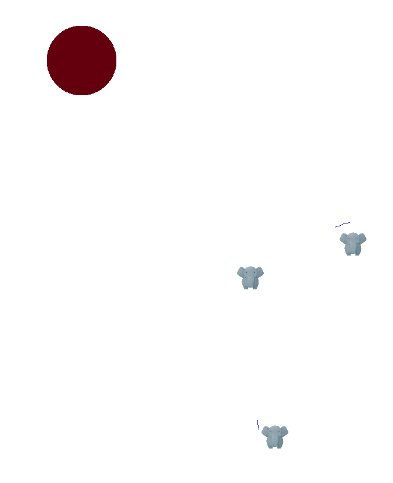
\includegraphics[scale=0.15]{eswsa1.png}
%			\captionof{figure}{ESWSA à l'itération 1}
%			\label{eswsa1}
%		\end{minipage}%

		\begin{minipage}{0.3\textwidth}
			\centering
			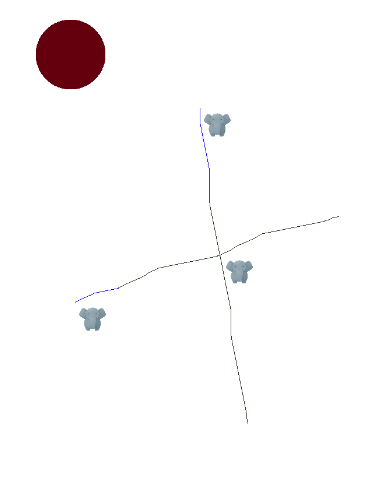
\includegraphics[width=0.9\textwidth]{eswsa4.png}
			\captionsetup{width=.9\linewidth}
			\captionof{figure}{ESWSA à l'itération 4}
			\label{eswsa4}
		\end{minipage}
		\hspace{0.2cm}
		\begin{minipage}{0.3\textwidth}
			\centering
			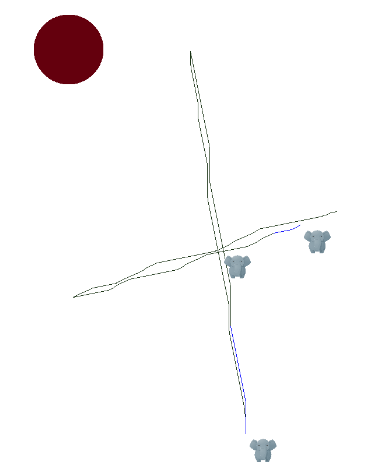
\includegraphics[width=0.9\textwidth]{eswsa8.png}
			\captionsetup{width=.9\linewidth}
			\captionof{figure}{ESWSA à l'itération 8}
			\label{eswsa8}
		\end{minipage}
		\hspace{0.2cm}
		\begin{minipage}{0.3\textwidth}
			\centering
			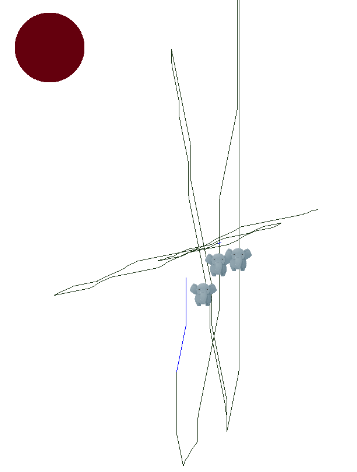
\includegraphics[width=0.89\textwidth]{eswsa16.png}
			\captionsetup{width=.9\linewidth}
			\captionof{figure}{ESWSA à l'itération 16}
			\label{eswsa16}
		\end{minipage}

	
	Par contre, une grande valeur de \textit{p} pousse les éléphants à suivre la même meilleure solution globale (\textit{Gbest}), convergeant ainsi vers une même cible ce qui cause un manque d'intensification.
	
	
	Le tableau suivant illustre les meilleurs paramètres obtenus pour l'algorithme ESWSA :
	\begin{table}[h]
		\begin{tabular}{|l|p{0.3cm}|p{0.3cm}|p{0.3cm}|p{0.3cm}|p{0.3cm}|p{0.3cm}|p{0.5cm}|p{0.5cm}|p{0.6cm}|p{0.5cm}|p{0.5cm}|p{0.6cm}|p{0.4cm}|p{0.4cm}|p{0.4cm}|}
			 \hline
			\multicolumn{1}{|c|}{\multirow{2}{*}{Type}} & \multicolumn{6}{c|}{Portée des cibles}                              & \multicolumn{6}{c|}{Taille d environnement}                         & \multicolumn{3}{l|}{\multirow{2}{*}{Nbr cibles}} \\ \cline{2-13}
			\multicolumn{1}{|c|}{}                      & \multicolumn{3}{c|}{mono-cible} & \multicolumn{3}{c|}{multi-cibles} & \multicolumn{3}{c|}{mono-cible} & \multicolumn{3}{c|}{multi-cibles} & \multicolumn{3}{l|}{}                            \\ \hline
			\multicolumn{1}{|c|}{Paramètres}            & 10        & 50       & 100      & 10         & 50        & 100      & 50        & 600      & 5000     & 50        & 600       & 5000      & 1              & 7              & 15             \\ \hline \hline
			nbrEle                                      & 16        & 15       & 10       & 19         & 17        & 14       & 12        & 14       & 19       & 16        & 16        & 18        & 17             & 15             & 20             \\ \hline
			Wt                                          & 0.4       & 0.5      & 0.4      & 0.4        & 0.5       & 0.3      & 0.6       & 0.5      & 0.5      & 0.6       & 0.5       & 0.5       & 0.5            & 0.4            & 0.5            \\ \hline
			p                                           & 0.6       & 0.5      & 0.3      & 0.5        & 0.5       & 0.5      & 0.5       & 0.5      & 0.3      & 0.6       & 0.5       & 0.5       & 0.5            & 0.5            & 0.5            \\ \hline
		\end{tabular}
		\caption{Meilleurs paramètres pour ESWSA.}
	\end{table}

	
	
%	\newpage
	
	%%%%%%%%%%%%%%%%%%%%%%%%%%%%%%%%%%%%%%%%%%%%%%%%%%%% %%%%%%%%%%%%%%%%%%%%%%%%%%%%%%%%%%%%%%%%%%%%%%%%%%%%
	%%%%%%%%%%%%%%%%%%%%%%%%%%%%%%%%%%%%%%%%%%%%%%%%%%%%
	\vspace{-0.5cm}
	
	\section{Expérimentations relatives à l'environnement}
	Nous avons sélectionné trois paramètres à expérimenter pour observer le comportement de nos approches de recherche basées essaims.
	Ces paramètres sont : \textit{la portée des cibles}, \textit{la taille de l'environnement} et \textit{le nombre de cibles recherchées}.
	
	Pour cela, nous avons réalisé ces expérimentations pour les trois types d'environnements précédemment explicités dans le chapitre 3, qui sont : \textbf{simples}, \textbf{avec obstacles} et \textbf{complexes}.
	
	

	

	
	\subsection{Organisation des types d'expérimentations}
	Pour une question de clarté, nous avons jugé nécessaire de décrire comment est organisé chaque type d'expérimentation avons de passer aux résultats obtenus.
	
	
	\subsubsection{Organisation des expérimentations par rapport à la portée des cibles}
	Pour les expérimentations relatives à l'influence de la portée des cibles sur le comportement de nos algorithmes de recherche, nous avons fixé la taille de l'environnement à 500 $\times$ 500 positions en faisant varier la portée d'un rayon de 10 positions à 100 positions avec un pas de 10.
	
	Ainsi comme le montre la figure \ref{orgPortee}, les tests de ce type proviennent des exécutions sur 40 environnements (4 par portée), ce qui fait 400 exécutions pour le mono-cible et 400 autres pour le multi-cibles, pour chaque méta-heuristique (après paramétrage).
	
	\begin{center}	 
		\captionsetup{width=1\linewidth} 
		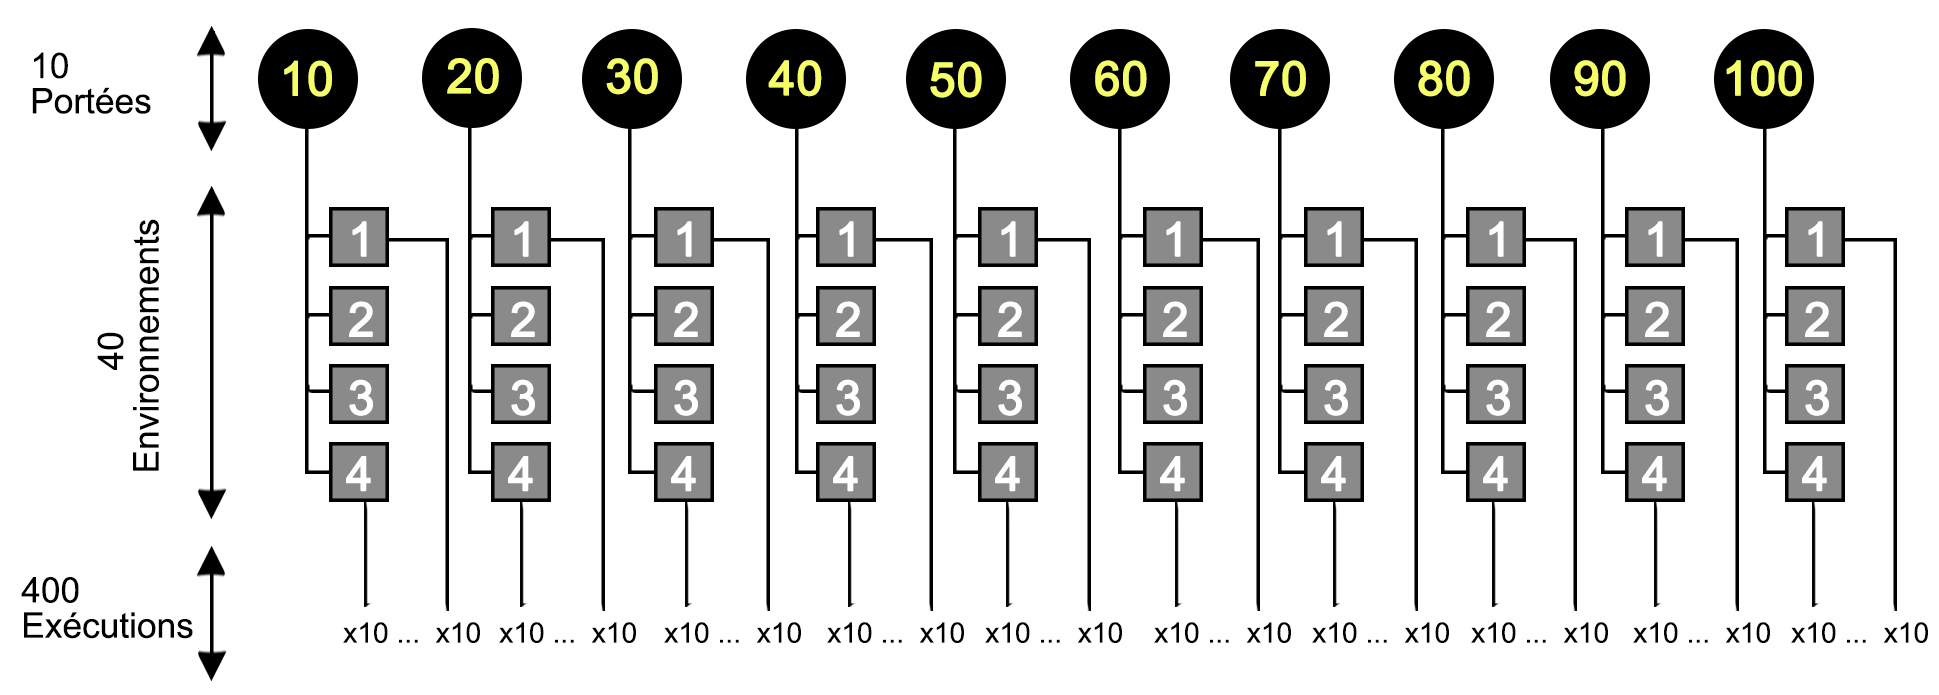
\includegraphics[width=0.7\textwidth]{org-portee.jpg}%
		\vspace{-0.1 cm}
		\captionof{figure}{Représentation de l'organisation des expérimentations sur la portée des cibles.}\label{orgPortee}%
	\end{center}
	
	\subsubsection{Organisation des expérimentations par rapport à la taille de l'environnement}
	Pour les expérimentations sur l'influence de la taille de l'environnement sur le comportement de nos méta-heuristiques à la recherche de cibles, nous avons adapté la portée des cibles à chaque taille d'environnement conformément à l'équation suivante :
	\begin{equation}
	portee = \frac{taille_{Cot\acute{e}} \times 10}{100} = \frac{taille_{Cot\acute{e}}}{10}
	\label{porteeEnv}
	\end{equation}	
	Ce qui revient à :
	\begin{equation}	
	S_{cible} = \frac{\sqrt{S_{env}}}{5} \times \pi
	\end{equation}
	
	Avec :
	\begin{itemize}
		\item[$-$] $taille_{Cot\acute{e}}$ : taille du coté de l'environnement carré.
		\item[$-$] $S_{cible}$ : surface d'émission de la cible (rayon = portée).
		\item[$-$] $S_{env}$ : surface de l'environnement de recherche ($S_{env}$ = $taille_{Cot\acute{e}}$).\\
	\end{itemize}
	
	Pour cela nous avons sélectionné dix différentes tailles d'environnement, les tailles du coté de ces environnements sont comme suit : 50, 100, 200, 400, 600, 800, 1000, 1500, 3000, 5000.
	
	Les surfaces respectives sont les suivantes: 2500, 10000, 40000, 160000, 360000, 640000, 1000000, 2250000, 9000000, 25000000.
	
	Les portées correspondantes sont: 5, 10, 20, 40, 60, 80, 100, 150, 300, 500.
	
	
	\textbf{ }\\
	Les résultats des tests liés à ce type d'expérimentation sont le résultat de 40 exécutions par taille d'environnement (4 configurations pour chaque taille), ce qui revient à un total de 400 exécutions pour le mono-cible et 400 autres pour le multi-cibles et ce pour chaque approche (après paramétrage). Le schéma \ref{orgSize} ci-dessous illustre cette organisation.
	
	\begin{center}	  
		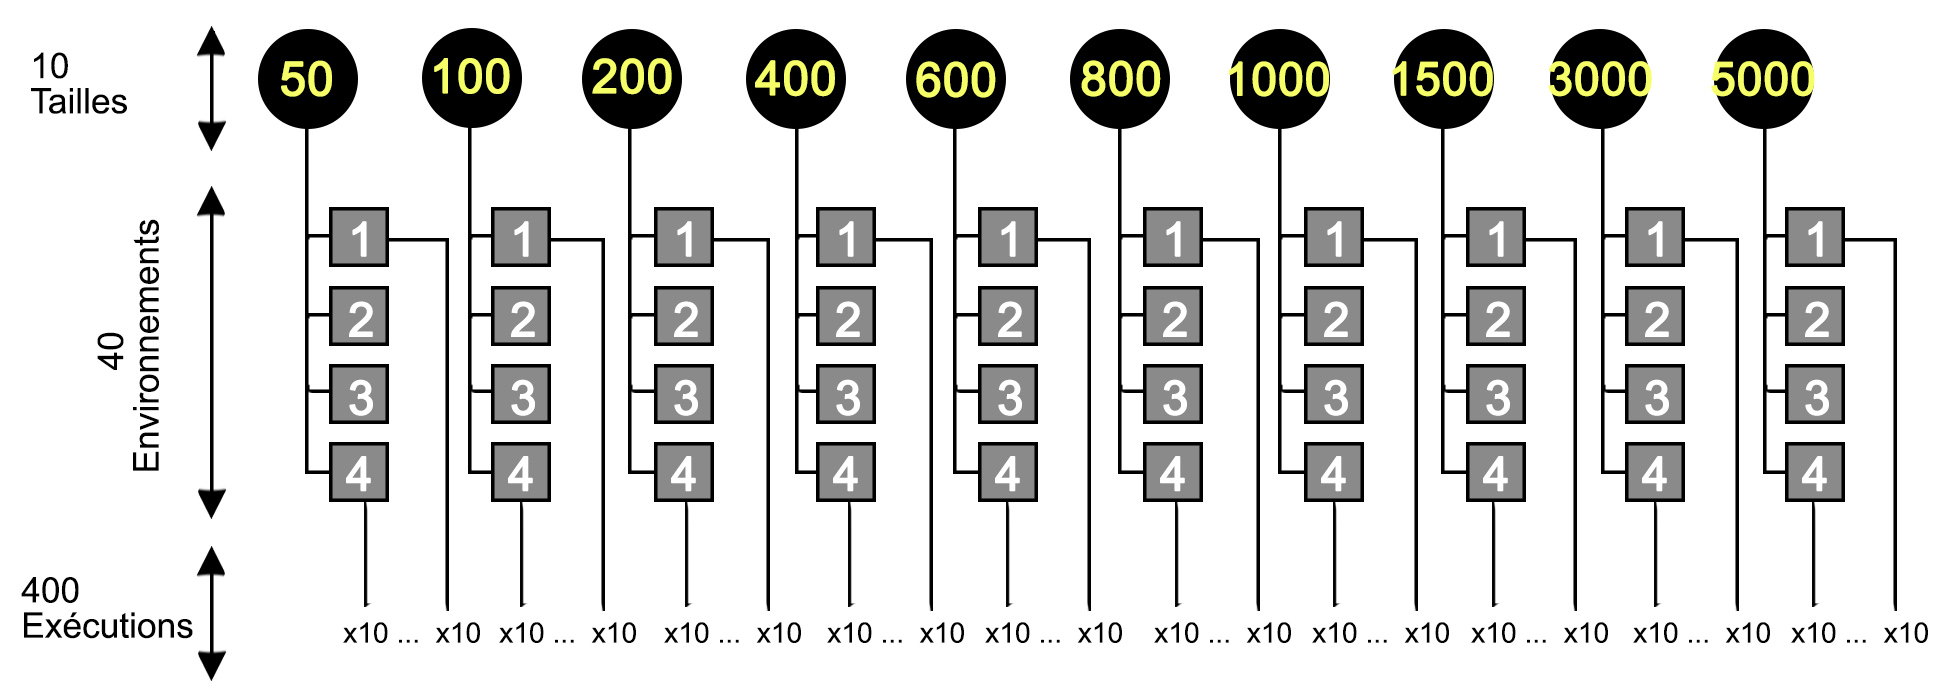
\includegraphics[width=0.75\textwidth]{org-size.jpg}%
		\vspace{-0.1 cm}
		\captionof{figure}{Représentation de l'organisation des expérimentations sur la taille des environnements.}\label{orgSize}%
	\end{center}
	
	\subsubsection{Organisation des expérimentations par rapport au nombre de cibles}
	Ces expérimentations permettent d'étudier l'impacte du changement du nombre de cibles présentes dans nos environnements sur le comportement de nos méta-heuristiques (BSO, EHO, ESWSA et Multi-BSO).
	Pour cela, nous avons fixé la taille des environnements à 500 $\times$ 500 positions ainsi qu'une portée de cible égale à 50 (Conformément à l'équation \ref{porteeEnv}).
	
	Nous avons pris le nombre de cibles compris entre 1 et 15 (bornes incluses) avec un pas de 2, ce qui nous donne les 8 nombres de cibles suivants : 1, 3, 5, 7, 9, 11, 13, 15.\\
	
	De ce fait, les résultats des tests sont le fruit d'exécutions sur 32 environnements (4 par nombre de cibles) , ce qui correspond à 320 exécutions pour chacune des approches développées (après paramétrage).\\
	La figure \ref{orgNbrT} ci-dessous schématise cette organisation :
	
	\begin{center}	  
		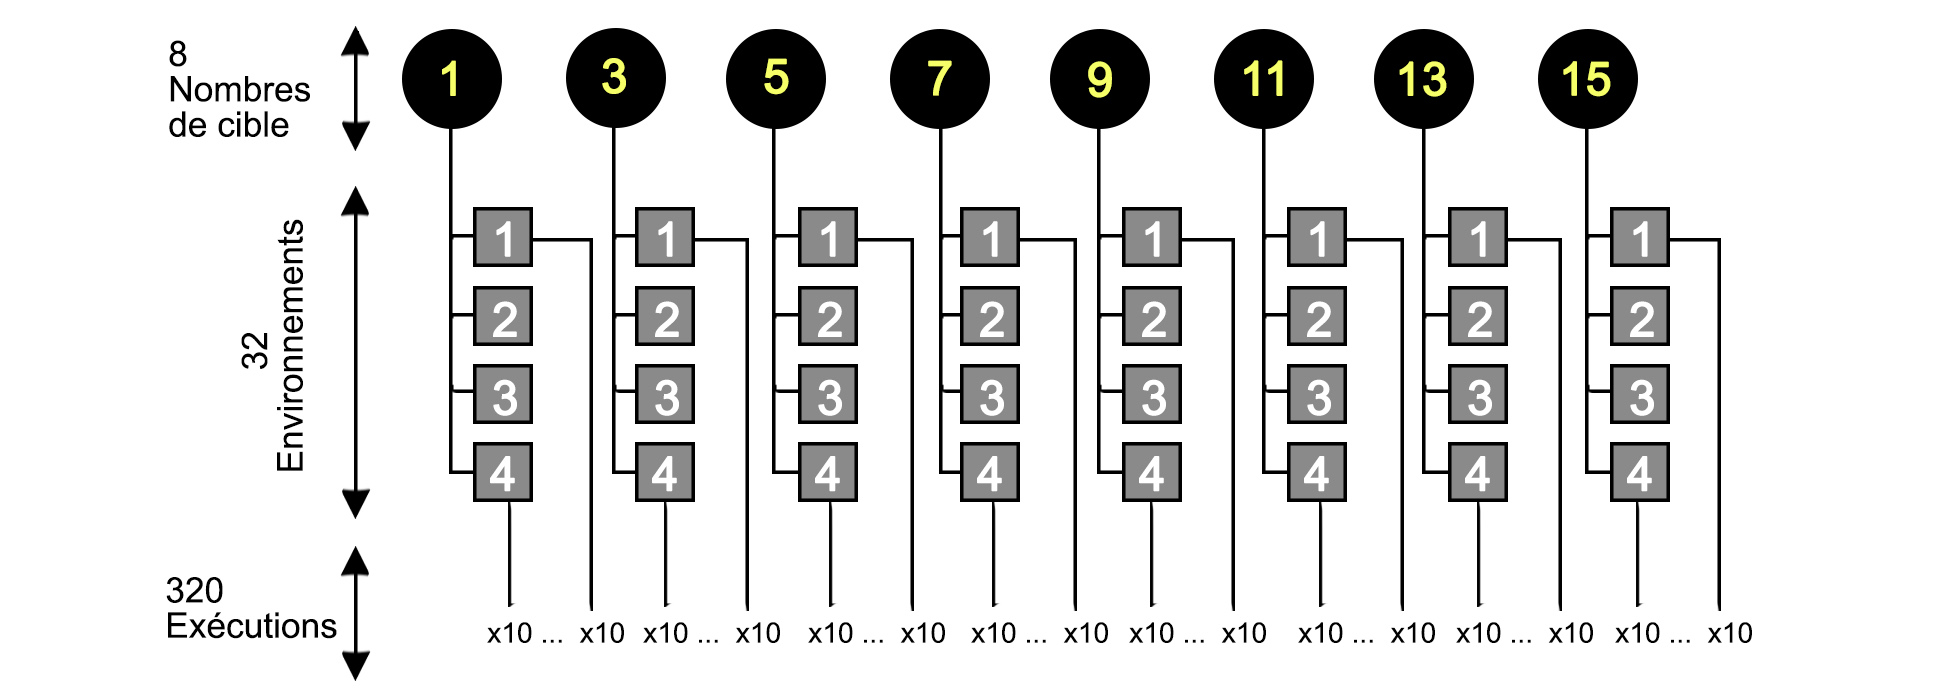
\includegraphics[width=0.8\textwidth]{org-nbrT.jpg}%
		\vspace{-0.1 cm}
		\captionof{figure}{Représentation de l'organisation des expérimentations sur le nombre de cibles.}\label{orgNbrT}%
	\end{center}
	
	
	

	%%%%%%%%%%%%%%%%%%%%%%%%%%%%%%%%%%%%%%%%%%%%%%%%%%%%%%
	%%%%%%%%%%%%%%%%%%%%%%%%%%%%%%%%%%%%%%%%%%%%%%%%%%%%%%\\
	%%%%%%%%%%%%%%%%%%%%%%%%%%%%%%%%%%%%%%%%%%%%%%%%%%%%%%\\
	
	
	\subsection{Expérimentations par rapport à la portée des cibles}
	
	\noindent
	\begin{minipage}[t]{0.5\textwidth}
		\subsubsection{Taux de réussite}
		
		La figure \ref{TP1} est un \textit{diagramme à bandes} représentant l'évolution du taux de réussite de chacune de nos méta-heuristiques par rapport aux différentes portées des cibles.\\
		
		Nous constatons que le taux de réussite est maximal (100\%) quelle que soit la valeur de la portée (de 10 à 100), autrement dit les algorithmes	implémentés arrivent toujours à trouver la ou les cible(s) sans atteindre le nombre maximal d'itérations qui est de 1000.
		
		Il est à noter que ces mêmes résultats ont été obtenus pour les trois types d'environnements (simple, avec obstacles et complexe) de dimensions 500 $\times$ 500 aussi bien dans les cas de mono-cible que de multi-cibles. 	
	\end{minipage}\hfill
	\begin{minipage}[t]{0.55\textwidth}
		\vspace{0.3cm}
		\captionsetup{width=0.8\linewidth}
		\centering\raisebox{\dimexpr \topskip-\height}{%
			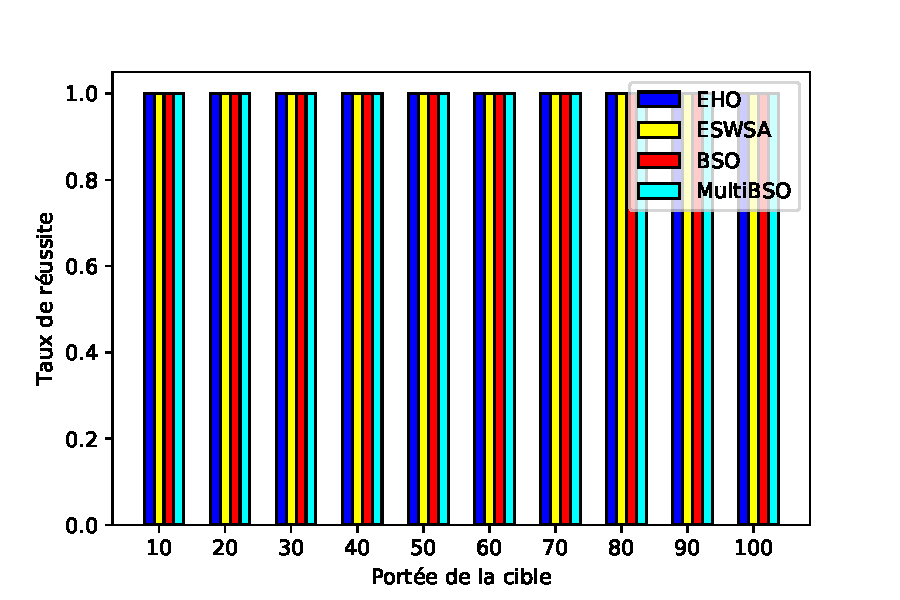
\includegraphics[width=\textwidth]{SansObs/BarChart/TauxPortee1.pdf}}
		\vspace{-0.3cm}
		\captionof{figure}{Comparaison de la variation du taux de réussite des algorithmes selon la portée des cibles.}
		\label{TP1}
	\end{minipage}\hfill
	
	
	\subsubsection{Variation du nombre d'itérations et temps d'exécution}
	\paragraph{a- Environnements simples (sans obstacles)}
	\paragraph{- Mono-cible}
	\vspace{-0.3cm}
	\textbf{ }\\
	Les figures \ref{IP1} et \ref{tP1} illustrent des \textit{diagrammes à lignes brisées}, représentant respectivement la variation du nombre d'itérations et temps d'exécution de chacune de nos approches confrontées aux différentes portées de la cible dans un environnement sans obstacle.\\
	\vspace{-0.2cm}
	
	On remarque que toutes les méthodes voient leur nombre d'itérations décroître avec l'élargissement de la portée de la cible. Pour les méthodes Multi-BSO, EHO et ESWSA, le nombre d'itérations est estimé entre 12 et 16 pour une portée égale à 10, puis décroît progressivement jusqu'à atteindre environ 2 ou 3 itérations pour la portée maximale. Quant à BSO, il débute avec un peu plus d'itérations (moyenne de 33), avant de diminuer pour rejoindre les autres méthodes lorsque la portée est maximale.\\
	\vspace{-0.2cm}
	
	Pour ce qui est des temps d'exécution, nos quatre méthodes s'exécutent en des temps records de moins de 0.08 secondes. BSO et Multi-BSO possèdent les meilleurs temps relativement stables et inférieurs à 0.02 secondes, suivies d'EHO atteignant les 0.05 secondes, enfin ESWSA est l'approche la plus lente en arrivant jusqu'à 0.08 secondes pour une portée égale à 100.
	
	\noindent
	\hspace{-0.5cm}
	\begin{minipage}[t]{0.55\textwidth}
		\captionsetup{width=0.8\linewidth}
		\centering\raisebox{\dimexpr \topskip-\height}{%
			\includegraphics[width=\textwidth]{SansObs/LineChart/IterPortee1.pdf}}
		\captionof{figure}{Comparaison de la variation du nombre d'itérations des algorithmes selon la portée de la cible (sans obstacles).}
		\label{IP1}
	\end{minipage}\hfill
	\hspace{-0.5cm}
	\begin{minipage}[t]{0.55\textwidth}
		\captionsetup{width=0.8\linewidth}
		\centering\raisebox{\dimexpr \topskip-\height}{%
			\includegraphics[width=\textwidth]{SansObs/LineChart/TimePortee1.pdf}}
		\captionof{figure}{Comparaison de la variation du temps d'exécution des algorithmes selon la portée de la cible (sans obstacles).}
		\label{tP1}
	\end{minipage}\hfill
	
	\paragraph{- Multi-cibles}
	\textbf{ }\\
	Les deux figures ci-dessous \ref{IP5} et \ref{tP5} sont représentatives de la variation du nombre d'itérations et temps d'exécution (dans cet ordre) de nos algorithmes, faces aux différentes portées des cibles dans des environnements sans obstacles.\\
	
	Nous distinguons trois comportements par rapport au nombre d'itérations, le premier est propre à BSO, celui-ci détient le plus grand nombre d'itérations pour toutes les portées, malgré la réduction de ce nombre de 107 à 29 en vue de l'augmentation des valeurs de la portée des cibles. 
	Compte au $2^{\grave{e}me}$, il est caractérisé par un nombre d'itérations avoisinant les 63 itérations pour une portée égale à 10, puis une diminution de ce nombre jusqu'à atteindre 8 à 4  itérations pour les cibles de portée 100; ce comportement concerne les deux méta-heuristiques EHO et ESWSA.
	Enfin, le $3^{\grave{e}me}$ comportement est celui de Multi-BSO, possédant le plus petit nombre d'itérations initial 31 qui diminue graduellement jusqu'à 9 itérations pour la portée égale à 100s.\\
	
	En termes de temps d'exécution, seul ESWSA subit une augmentation visible allant de 0.15 à 0.83 secondes pour les portées de 10 à 100 respectivement,  les trois autres algorithmes ne dépassent pas les 0.23 secondes, cette valeur correspondant aux résultats d'EHO pour la portée de 100 positions, BSO et Multi-BSO ayant des temps légèrement inférieurs.
	
	\noindent
	\hspace{-0.5cm}
	\begin{minipage}[t]{0.55\textwidth}
		\captionsetup{width=0.8\linewidth}
		\centering\raisebox{\dimexpr \topskip-\height}{%
			\includegraphics[width=\textwidth]{SansObs/LineChart/IterPortee5.pdf}}
		\captionof{figure}{Comparaison de la variation du nombre d'itérations des algorithmes selon la portée des cibles (sans obstacles).}
		\label{IP5}
	\end{minipage}\hfill
	\hspace{-0.5cm}
	\begin{minipage}[t]{0.55\textwidth}
		\captionsetup{width=0.8\linewidth}
		\centering\raisebox{\dimexpr \topskip-\height}{%
			\includegraphics[width=\textwidth]{SansObs/LineChart/TimePortee5.pdf}}
		\captionof{figure}{Comparaison de la variation du temps d'exécution des algorithmes selon la portée des cibles (sans obstacles).}
		\label{tP5}
	\end{minipage}\hfill
	
	
	\paragraph{b- Environnements avec obstacles}
	\paragraph{- Mono-cible}
	\textbf{ }\\
	Les deux \textit{diagrammes à lignes brisées} des figures \ref{IP1o} et \ref{tP1o} retracent la variation du nombre moyen d'itérations et temps moyens d'exécution de nos algorithmes faisant face à une portée croissante de la cible dans des environnements avec obstacles.\\
	\vspace{-0.2cm}
	
	Pour la première valeur de portée (égale à 10) l'approche BSO est celle qui nécessite le plus d'itérations (52.68), suivie d'EHO et Multi-BSO dont le nombre d'itérations est d'environ 14, enfin ESWSA, qui démarre avec seulement 3.58 itérations. 
	
	Pour toutes les méta-heuristiques, ce nombre évolue de manière inversement proportionnelle à la portée de la cible jusqu'à ce que la portée soit égale à 50 où il commence à se stabiliser autour de 9 itérations.\\
	\vspace{-0.2cm}
	
	Les temps d'exécution sont minorés par 0.001 secondes et majorés par la valeur 0.11 secondes, ce qui est remarquablement rapide. On distingue une augmentation des temps d'exécution pour ESWSA, plus légère pour EHO suite à l'élargissement de la surface de la portée de la cible. Les deux autres approches restent moyennement stables n'excédant pas les 0.02 secondes.   
	
	
	\vspace{-0.1cm}
	\noindent
	\hspace{-0.5cm}
	\begin{minipage}[t]{0.55\textwidth}
		\captionsetup{width=0.8\linewidth}
		\centering\raisebox{\dimexpr \topskip-\height}{%
			\includegraphics[width=\textwidth]{AvecObs/LineChart/IterPortee1.pdf}}
		\captionof{figure}{Comparaison de la variation du nombre d'itérations des algorithmes selon la portée de la cible (avec obstacles).}
		\label{IP1o}
	\end{minipage}\hfill
	\hspace{-0.5cm}
	\begin{minipage}[t]{0.55\textwidth}
		\captionsetup{width=0.8\linewidth}
		\centering\raisebox{\dimexpr \topskip-\height}{%
			\includegraphics[width=\textwidth]{AvecObs/LineChart/TimePortee1.pdf}}
		\captionof{figure}{Comparaison de la variation du temps d'exécution des algorithmes selon la portée de la cible (avec obstacles).}
		\label{tP1o}
	\end{minipage}\hfill
	
	
	\paragraph{- Multi-cibles}
	\textbf{ }\\
	Les figures \ref{IP5o} et \ref{tP5o} reflètent la variation du nombre d'itérations et temps d'exécution de nos quatre approches de recherche face aux portées des cibles, cela dans des environnements avec obstacles.\\
	
	Le nombre d'itérations diminue avec l'augmentation de la portée des cibles pour toutes les approches, néanmoins BSO se distingue par une diminution importante en passant d'une moyenne de 110.6 à 22.58 itérations. Contrairement à Multi-BSO, EHO et ESWSA qui varient entre 30 et 3 itérations.\\
	
	Pour ce qui est des temps d'exécution, nous remarquons que pour ESWSA la durée de recherche croît considérablement avec l'augmentation de la portée des cibles, comme nous pouvons le voir, il passe de 0.06 à 2.73 secondes. Les autres algorithmes qui se comportent de manière similaire, mais avec une marge moins importante passant de 0.01 à 0.23 secondes.
	
	
	\noindent
	\hspace{-0.5cm}
	\begin{minipage}[t]{0.55\textwidth}
		\captionsetup{width=0.8\linewidth}
		\centering\raisebox{\dimexpr \topskip-\height}{%
			\includegraphics[width=\textwidth]{AvecObs/LineChart/IterPortee5.pdf}}
		\captionof{figure}{Comparaison de la variation du nombre d'itérations des algorithmes selon la portée des cibles (avec obstacles).}
		\label{IP5o}
	\end{minipage}\hfill
	\hspace{-0.5cm}
	\begin{minipage}[t]{0.55\textwidth}
		\captionsetup{width=0.8\linewidth}
		\centering\raisebox{\dimexpr \topskip-\height}{%
			\includegraphics[width=\textwidth]{AvecObs/LineChart/TimePortee5.pdf}}
		\captionof{figure}{Comparaison de la variation du temps d'exécution des algorithmes selon la portée des cibles. (avec obstacles)}
		\label{tP5o}
	\end{minipage}\hfill
	
	
	\paragraph{c- Environnements complexes}
	\paragraph{- Mono-cible}
	\textbf{ }\\
	Les \textit{diagrammes à lignes brisées} des figures \ref{IP1c} et \ref{tP1c}, décrivent la variation du nombre d'itérations et temps d'exécution de nos approches, celles-ci confrontées aux diverses valeurs de portée de la cible recherchée et cela, dans des environnements complexes.\\
	
	Nous remarquons que le nombre d'itérations décroît avec l'augmentation de la portée de la cible, BSO débute avec le plus grand nombre de 60.83 pour en effectuer que 6.60 itérations lorsque la portée est à 100. ESWSA passe de 40.08 à 2.03 itérations. Quant à EHO, lui fluctue entre 22.13 et 1.48 itérations. Enfin Multi-BSO possède la courbe descendante la plus régulière qui passe de 25 à 3.05 itérations.\\
	
	Pour ce qui est des temps d'exécution, ceux de BSO, Multi-BSO ainsi qu'EHO connaissent une légère augmentation de 0.02 à 0.04 secondes contrairement à ceux d'ESWSA qui double passant de 0.06 à 0.12 secondes.
	
	
	
	\noindent
	\hspace{-0.5cm}
	\begin{minipage}[t]{0.55\textwidth}
		\captionsetup{width=0.8\linewidth}
		\centering\raisebox{\dimexpr \topskip-\height}{%
			\includegraphics[width=\textwidth]{Complex/LineChart/IterPortee1.pdf}}
		\captionof{figure}{Comparaison de la variation du nombre d'itérations des algorithmes selon la portée de la cible (complexe).}
		\label{IP1c}
	\end{minipage}\hfill
	\begin{minipage}[t]{0.55\textwidth}
		\centering\raisebox{\dimexpr \topskip-\height}{%
			\includegraphics[width=\textwidth]{Complex/LineChart/TimePortee1.pdf}}
		\captionof{figure}{Comparaison de la variation du temps d'exécution des algorithmes selon la portée de la cible (complexe).}
		\label{tP1c}
	\end{minipage}\hfill
	
	\paragraph{- Multi-cibles}
	\textbf{ }\\
	\'{A} travers les figures \ref{IP5c} et \ref{tP5c}, sont représentées respectivement la variation du nombre d'itérations et temps d'exécution de nos approches sous-mises aux dix valeurs de portée des cibles dans des environnements complexes.\\
	
	Comme dans le mode mono-cible, l'augmentation de la portée des cibles conduit à une baisse du nombre d'itérations. On note pour la méta-heuristique BSO une importante chute du nombre d'itérations allant de 110.6 à 22.58 suivie d'EHO et Multi-BSO qui se comportent de façon similaire avec un nombre d'itérations initial aux alentours de 80 qui dégringole aux environs de 8 itérations. Enfin, ESWSA possède la baisse la moins flagrante, passant de 46.88 à 3.08 itérations atteignant le nombre minimum d'itérations qui est de 3.\\
	
	Une hausse du taux de croissance est observée pour les temps d'exécution d'ESWSA (de 0.05 à 1.10 secondes). Contrairement à ceux de BSO, Multi-BSO et EHO où une stabilisation demeure avec une très légère augmentation pour EHO ne dépassant pas les 0.21 secondes, pour les portées entre 60 et 100.
	
	
	
	\noindent
	\hspace{-0.5cm}
	\begin{minipage}[t]{0.55\textwidth}
		\captionsetup{width=0.8\linewidth}
		\centering\raisebox{\dimexpr \topskip-\height}{%
			\includegraphics[width=\textwidth]{Complex/LineChart/IterPortee5.pdf}}
		\captionof{figure}{Comparaison de la variation du nombre d'itérations des algorithmes selon la portée des cibles (complexe).}
		\label{IP5c}
	\end{minipage}\hfill
	\hspace{-0.5cm}
	\begin{minipage}[t]{0.55\textwidth}
		\captionsetup{width=0.8\linewidth}
		\centering\raisebox{\dimexpr \topskip-\height}{%
			\includegraphics[width=\textwidth]{Complex/LineChart/TimePortee5.pdf}}
		\captionof{figure}{Comparaison de la variation du temps d'exécution des algorithmes selon la portée des cibles (complexe).}
		\label{tP5c}
	\end{minipage}\hfill
	
	
	\subsubsection{- Analyse relative à la portée des cibles}
	
	À travers les résultats commentés des cas du mono-cible et multi-cibles appliqués à toutes les approches, on peut retenir les points suivants :
	
	\begin{itemize}
		\item[$\bullet$] Même pour de petites portées des cibles, nos algorithmes arrivent à bout de la recherche avec succès.
		
		\item[$\bullet$] L'élargissement graduel de la portée des cibles a fait fléchir le nombre d'itérations.
		
		\item[$\bullet$] Malgré les temps d'exécution acceptables, ils sont moyennement plus importants pour le mode multi-cibles.
		
		\item[$\bullet$] La densité des obstacles influe la recherche, ce qui s'explique par l'augmentation des temps d'exécution et nombre d'itérations.\\
	\end{itemize}
	
	%%%%%%%%%%%%%%%%%%%%%%%%%%%%%%%%%%%%%%%%%%%%%%%%%%%%%%%%%%%%%%%%%%%%%%%%%%%%%%%%%%%%%%%%%%%%%%%%%%%%%%%%%%%%%%%%%%%%%%%%%%%%%%%%%%%%%%%%%%%%%%%%%%%%%%%%%%%%%%%%%%
	
	\subsection{Expérimentations par rapport à la taille de l'environnement}
	
	\subsubsection{Taux de réussite}
	\textbf{}
	
	\paragraph{a- Environnements simples (sans obstacles)}
	\textbf{}\\
	\noindent
	\begin{minipage}[t]{0.5\textwidth}
		\paragraph{- Mono-cible}
		\textbf{}\\
		Le graphe de la figure \ref{TS1} montre la variation du taux de réussite pour chaque approche développée, celles-ci sous-mises à diverses tailles d'environnements sans obstacles.\\
		
		Pour EHO et ESWSA, un taux maximal de réussite est observé quelle que soit la taille de l'environnement. En revanche, BSO et Multi-BSO voient leur taux de succès maximal diminuer jusqu'à 60\% pour BSO et 77\% pour Multi-BSO pour les deux dernières tailles c'est-à-dire 3000 et 5000.
		
		
		
	\end{minipage}\hfill
	\begin{minipage}[t]{0.55\textwidth}
		\captionsetup{width=0.8\linewidth}
		\centering\raisebox{\dimexpr \topskip-\height}{%
			\includegraphics[width=\textwidth]{SansObs/BarChart/TauxSize1.pdf}}
		\captionof{figure}{Comparaison de la variation du taux de réussite des algorithmes selon la taille de l'environnement (sans obstacles).}
		\label{TS1}
	\end{minipage}\hfill
	
	\textbf{ }
	
	\noindent
	\begin{minipage}[t]{0.5\textwidth}
		\paragraph{- Multi-cibles}
		\textbf{}\\
		La figure \ref{TS5} à droite décrit les taux de réussite dans la recherche des cibles, de chaque méta-heuristique en fonction de la variation de la taille des environnements sans obstacles.\\
		Nous nous apercevons que comme pour le mono-cible, EHO et ESWSA atteignent le taux de 100\% pour toutes les tailles, ce qui n'est pas le cas de BSO dont le taux de réussite décroît à partir de la $7^{\grave{e}me}$ taille d'environnement avec 99\% pour atteindre 51\% pour les environnements de taille 5000 et Multi-BSO dont les taux de succès des deux dernières tailles d'environnement sont respectivement de 85\% et 79\%.
		
	\end{minipage}\hfill
	\begin{minipage}[t]{0.55\textwidth}
		\captionsetup{width=0.8\linewidth}
		\centering\raisebox{\dimexpr \topskip-\height}{%
			\includegraphics[width=\textwidth]{SansObs/BarChart/TauxSize5.pdf}}
		\captionof{figure}{Comparaison de la variation du taux de réussite des algorithmes selon la taille de l'environnement (sans obstacles).}
		\label{TS5}
	\end{minipage}\hfill
	
	
	\paragraph{b- Environnements avec obstacles}
	\textbf{}\\
	\noindent
	\begin{minipage}[t]{0.5\textwidth}
		\paragraph{- Mono-cible}
		\textbf{}\\
		La figure \ref{TS1o} affiche la variation des taux de réussite de nos approches selon des tailles croissantes des environnements avec obstacles.\\
		
		Pour les tailles entre 50 et 1 500, tous nos algorithmes arrivent à obtenir les 100\% de taux de succès, toutefois les environnements de dimensions 3 000  connaissent une baisse de ce taux à 76\% pour BSO, mais toujours 100\% pour les autres. Enfin, pour les plus grands environnements Multi-BSO atteint un taux de 87\% contre 55\% pour BSO et 100\% pour EHO et ESWSA. 
		
		
		
	\end{minipage}\hfill
	\begin{minipage}[t]{0.55\textwidth}
		\captionsetup{width=0.8\linewidth}
		\centering\raisebox{\dimexpr \topskip-\height}{%
			\includegraphics[width=\textwidth]{AvecObs/BarChart/TauxSize1.pdf}}
		\captionof{figure}{Comparaison de la variation du taux de réussite des algorithmes selon la taille de l'environnement (avec obstacles).}
		\label{TS1o}
	\end{minipage}\hfill
	
	
	
	\noindent
	\begin{minipage}[t]{0.50\textwidth}
		\paragraph{- Multi-cibles}
		\textbf{}
		
		La figure \ref{TS5o} représente la variation des taux de succès de nos approches confrontées à plusieurs tailles d'environnement avec obstacles.\\
		
		EHO et ESWSA arrivent à maintenir les 100\% de taux de réussite pour toutes les tailles testées, contrairement à Multi-BSO qui relâche son taux de réussite à 83\% au bout de l'avant-dernière taille (3 000), et BSO qui déjà à partir des tailles 1 000 baisse à 67\% pour continuer à baisser jusqu'à 17\%. Toujours dans la limite du nombre d'itérations maximal (1 000).
		
	\end{minipage}\hfill
	\begin{minipage}[t]{0.55\textwidth}
		\captionsetup{width=0.8\linewidth}
		\centering\raisebox{\dimexpr \topskip-\height}{%
			\includegraphics[width=\textwidth]{AvecObs/BarChart/TauxSize5.pdf}}
		\captionof{figure}{Comparaison de la variation du taux de réussite des algorithmes selon la taille de l'environnement (avec obstacles).}
		\label{TS5o}
	\end{minipage}\hfill
	
	\textbf{ }
	\paragraph{c- Environnements complexes}
	\textbf{}\\
	\noindent
	\begin{minipage}[t]{0.5\textwidth}
		\paragraph{- Mono-cible}
		\textbf{}
		
		Dans la figure \ref{TS1c} est représentée la variation des taux de réussite de l'ensemble de nos approches exécutées sur différentes tailles d'environnements complexes.\\
		
		Pour toutes les tailles testées de 50 à 3 000 la totalité de nos algorithmes atteignent les 100\% de réussite, mais pour la dernière taille d'environnement (5 000) seuls EHO et ESWSA arrivent à garder le même taux de réussite, tels que Multi-BSO décent à 90\% et BSO chute à 60\%, car ils sont limités par le nombre d'itérations maximal.
		
	\end{minipage}\hfill
	\begin{minipage}[t]{0.55\textwidth}
		\captionsetup{width=0.8\linewidth}
		\centering\raisebox{\dimexpr \topskip-\height}{%
			\includegraphics[width=\textwidth]{SansObs/BarChart/TauxSize1.pdf}}
		\captionof{figure}{Comparaison de la variation du taux de réussite des algorithmes selon la taille de l'environnement (complexe).}
		\label{TS1c}
	\end{minipage}\hfill
	
	
	\noindent
	\begin{minipage}[t]{0.5\textwidth}
		\paragraph{- Multi-cibles}
		\textbf{}
		
		Les \textit{diagrammes à bandes} de la figure \ref{TS5c} décrivent comment les taux de succès de nos algorithmes varient faces aux tailles d'environnements complexes à la recherche de plusieurs cibles.\\
		
		EHO et ESWSA maintiennent les 100\% de taux de réussite pour toutes les tailles d'environnement, idem pour Multi-BSO sauf pour ce qui est de la dernière taille, il n'arrive qu'à 71\%. Par contre BSO décent sous la barre des 100\% dès la taille 1000, à partir de là, son taux fluctue entre 36\% et 98\% car freiné par le nombre d'itérations maximal.
		
	\end{minipage}\hfill
	\begin{minipage}[t]{0.55\textwidth}
		%\vspace{0.2cm}
		\captionsetup{width=0.8\linewidth}
		\centering\raisebox{\dimexpr \topskip-\height}{%
			\includegraphics[width=\textwidth]{Complex/BarChart/TauxSize5.pdf}}
		\captionof{figure}{Comparaison de la variation du taux de réussite des algorithmes selon la taille de l'environnement (complexe).}
		\label{TS5c}
	\end{minipage}\hfill
	
	
	
	\subsubsection{Variation du nombre d'itérations et temps d'exécution}
	\paragraph{a- Environnements simples (sans obstacles)}
	\textbf{}
	\vspace{-0.3cm}
	\noindent
	\paragraph{- Mono-cible}
	\textbf{ }
	
	Dans les figures \ref{IS1} et \ref{tS1} sont représentés la variation du nombre d'itérations et du temps d'exécution de nos méta-heuristiques pour l'ensemble des tailles d'environnement sans obstacles sélectionnées.\\
	\vspace{-0.2cm}
	
	Les méta-heuristiques inspirées des éléphants détiennent le nombre d'itérations le plus réduit, celui-ci varie entre 1 et 10 itérations pour EHO et entre 2 et 13 itérations pour ESWSA. Par contre, les deux variantes de BSO connaissent une importante augmentation du nombre d'itérations de 4 à 574 itérations pour BSO et de 2 à 189 pour Multi-BSO, suite à l'augmentation de la taille des environnements.\\
	\vspace{-0.2cm}
	
	Pour ce qui est de l'aspect "temps", toutes les approches sont sujettes à une croissance proportionnelle à la croissance des tailles d'environnement à différents coefficients près, tels que nous pouvons les ordonner selon la vitesse d'augmentation des temps d'exécution de l'algorithme le plus lent au plus rapide comme suit : ESWSA puis BSO suivis de Multi-BSO et enfin EHO, ce dernier atteint un maximum de 4.6 secondes pour une taille = 5 000.
	
	\noindent
	\hspace{-0.5cm}
	\begin{minipage}[t]{0.55\textwidth}
		\captionsetup{width=0.8\linewidth}
		\centering\raisebox{\dimexpr \topskip-\height}{%
			\includegraphics[width=\textwidth]{SansObs/LineChart/IterSIze1.pdf}}
		\captionof{figure}{Comparaison de la variation du nombre d'itérations des algorithmes selon la taille de l'environnement (sans obstacles).}
		\label{IS1}
	\end{minipage}\hfill
	\hspace{-0.5cm}
	\begin{minipage}[t]{0.55\textwidth}
		\captionsetup{width=0.8\linewidth}
		\centering\raisebox{\dimexpr \topskip-\height}{%
			\includegraphics[width=\textwidth]{SansObs/LineChart/TimeSIze1.pdf}}
		\captionof{figure}{Comparaison de la variation du temps d'exécution des algorithmes selon la taille de l'environnement (sans obstacles).}
		\label{tS1}
	\end{minipage}\hfill
	
	
	\noindent
	\paragraph{- Multi-cibles}
	\textbf{ }
	
	Les courbes des figures \ref{IS5} et \ref{tS5} illustrent la variation du nombre moyen d'itérations et temps moyens d'exécution de nos algorithmes vis-à-vis des différentes tailles d'environnement sans obstacles.\\
	\vspace{-0.2cm}
	
	Ici aussi, pour le mode multi-cibles EHO et ESWSA effectuent le moins d'itérations, avec une légère augmentation allant de 2.43 jusqu'à 19.43 itérations pour EHO, de 3.73 à 6.95 itérations pour ESWSA, cela pour l'agrandissement de la taille des environnements.
	Par ailleurs, BSO et Multi-BSO subissent une conséquente élévation du nombre d'itérations allant de 9.88 à 991.18 itérations pour BSO et de 5.95 à 865.53 pour ce qui est de Multi-BSO.\\
	\vspace{-0.2cm}
	
	Quant aux temps d'exécution, globalement nous pouvons dire que les temps d'exécution des algorithmes croient avec l'augmentation de la taille des environnements à différentes vitesses, tels que BSO passe progressivement de 0.001 à 6.57 secondes suivi de Multi-BSO avec des temps haussant de 0.001 à 11.75 secondes, puis EHO qui démarre à 0.001 pour atteindre les 19.43 secondes et enfin ESWSA qui enregistre les plus grands temps passant de  0.001 à 17.01 secondes.
	
	
	
	\noindent
	\begin{minipage}[t]{0.55\textwidth}
		\hspace{-0.5cm}
		\captionsetup{width=0.8\linewidth}
		\centering\raisebox{\dimexpr \topskip-\height}{%
			\includegraphics[width=\textwidth]{SansObs/LineChart/IterSIze5.pdf}}
		\captionof{figure}{Comparaison de la variation du nombre d'itérations des algorithmes selon la taille de l'environnement (sans obstacles).}
		\label{IS5}
	\end{minipage}\hfill
	\hspace{-0.5cm}
	\begin{minipage}[t]{0.55\textwidth}
		\captionsetup{width=0.8\linewidth}
		\centering\raisebox{\dimexpr \topskip-\height}{%
			\includegraphics[width=\textwidth]{SansObs/LineChart/TimeSIze5.pdf}}
		\captionof{figure}{Comparaison de la variation du temps d'exécution des algorithmes selon la taille de l'environnement (sans obstacles).}
		\label{tS5}
	\end{minipage}\hfill
	
	\paragraph{b- Environnements avec obstacles}
	\textbf{}
	\noindent
	\paragraph{- Mono-cible}
	\textbf{ }
	
	Les \textit{diagrammes à lignes brisées} des figures \ref{IS1o} et \ref{tS1o} font apparaître la variation du nombre d'itérations et temps d'exécution de BSO, Multi-BSO, EHO ainsi qu'ESWSA par rapport aux tailles des environnements avec obstacles.\\
	\vspace{-0.2cm}
	
	La figure de gauche montre que BSO détient le plus grand nombre d'itérations pour l'ensemble des tailles d'environnement, avec une augmentation allant de 2.55 à 566.18 itérations. Multi-BSO vient juste après avec des nombres d'itérations croissants tout en restant réduit jusqu'aux environnements de 3000 $\times$ 3000 où il arrive à 48.45 itérations qui par la suite grimpe vers 295.58 itérations pour les plus grands environnements.
	Enfin, EHO et ESWSA disposent des nombres d'itérations les plus réduis, fluctuant entre 1.08 et 29.78 itérations.\\
	\vspace{-0.2cm}
	
	Quant à la figure de droite, nous y discernons deux comportements tous deux croissants avec l'élargissement des surfaces des environnements, le $1^{er}$ englobe BSO, Multi-BSO et EHO qui possèdent des temps d'exécution minimes (entre 0.001 et 3.83 secondes), et le $2^{\grave{e}me}$ comportement concerne ESWSA avec des temps moyens plus ou moins élevés, allant de 0.001 à 15.56 secondes.
	
	
	
	\noindent
	\hspace{-0.3cm}
	\begin{minipage}[t]{0.55\textwidth}
		\captionsetup{width=0.8\linewidth}
		\centering\raisebox{\dimexpr \topskip-\height}{%
			\includegraphics[width=\textwidth]{AvecObs/LineChart/IterSIze1.pdf}}
		\captionof{figure}{Comparaison de la variation du nombre d'itérations des algorithmes selon la taille de l'environnement (avec obstacles).}
		\label{IS1o}
	\end{minipage}\hfill
	\hspace{-0.5cm}
	\begin{minipage}[t]{0.55\textwidth}
		\captionsetup{width=0.8\linewidth}
		\centering\raisebox{\dimexpr \topskip-\height}{%
			\includegraphics[width=\textwidth]{AvecObs/LineChart/TimeSIze1.pdf}}
		\captionof{figure}{Comparaison de la variation du temps d'exécution des algorithmes selon la taille de l'environnement (avec obstacles).}
		\label{tS1o}
	\end{minipage}\hfill
	
	\noindent
	\paragraph{- Multi-cibles}
	\textbf{ }
	
	Les figures \ref{IS5o} et \ref{tS5o} présentées ci-dessous, retracent la variation du nombre d'itérations et temps d'exécution de nos algorithmes testés sur plusieurs tailles d'environnement avec obstacles à la recherche de plusieurs cibles.\\
	\vspace{-0.2cm}
	
	BSO et Multi-BSO se distinguent avec des nombres élevés d'itérations, BSO débutant de 9.50 itérations et arrivant à la limite maximale de 1000 itérations, quant à Multi-BSO il passe d'une moyenne de 5.40 à 920.68 itérations. D'autre part EHO et ESWSA possèdent le moins d'itérations (entre 2.45 et 22.18 itérations).\\
	\vspace{-0.2cm}	
	
	Côté temps d'exécution, nous pouvons ordonner nos méthodes de la plus rapide à la plus long comme suit : BSO avec de 0.001 à 1.99 secondes suivie de Multi-BSO avec de 0.01 à 5.67 secondes puis EHO avec des temps entre 2.45 et 20.50 secondes, pour finir ESWSA dont les temps croissent de manière spectaculaire de 0.001 à 94.55 secondes. 
	
	
	
	\noindent
	\hspace{-0.5cm}
	\begin{minipage}[t]{0.55\textwidth}
		\captionsetup{width=0.8\linewidth}
		\centering\raisebox{\dimexpr \topskip-\height}{%
			\includegraphics[width=\textwidth]{AvecObs/LineChart/IterSIze5.pdf}}
		\captionof{figure}{Comparaison de la variation du nombre d'itérations des algorithmes selon la taille de l'environnement (avec obstacles).}
		\label{IS5o}
	\end{minipage}\hfill
	\hspace{-0.5cm}
	\begin{minipage}[t]{0.55\textwidth}
		\captionsetup{width=0.8\linewidth}
		\centering\raisebox{\dimexpr \topskip-\height}{%
			\includegraphics[width=\textwidth]{AvecObs/LineChart/TimeSIze5.pdf}}
		\captionof{figure}{Comparaison de la variation du temps d'exécution des algorithmes selon la taille de l'environnement (avec obstacles).}
		\label{tS5o}
	\end{minipage}\hfill
	
	
	
	\paragraph{c- Environnements complexes}
	\textbf{}
	\noindent
	\paragraph{- Mono-cible}
	\textbf{ }\\
	Dans les figures \ref{IS1c} et \ref{tS1c} sont décrites la variation du nombre d'itérations et celle du temps d'exécution de nos algorithmes selon la taille des environnements complexes.\\
	\vspace{-0.2cm}
	
	Nous pouvons regrouper les méta-heuristiques en deux groupes d'après l'évolution de leur nombre d'itérations, le $1^{er}$ groupe est constitué de BSO et Multi-BSO qui subit une importante croissance de ce nombre passant de 2.7 à 747.78 itérations pour BSO et de 2.05 à 444.45 itérations pour Multi-BSO.
	
	Le $2^{\grave{e}me}$ groupe est celui d'EHO et ESWSA, ceux-ci croient de manière bien plus raisonnable, soient de 1.35 à 13.83 itérations pour EHO et de 1.05 à 70.45 itérations pour ESWSA.\\
	\vspace{-0.2cm}
	
	Toutes nos approches connaissent un 
	accroissement des temps d'exécution avec l'élargissement des tailles d'environnement. ESWSA est celle dont les temps ont le plus augmenté (de 0.001 à 12.32 secondes), suivie d'EHO avec des temps qui passent de 0.001 à 3.03 secondes, puis vient Multi-BSO avec entre 0.001 et 1.92 secondes. Enfin, la plus rapide est BSO, dont les temps sont entre 0.001 et 1 seconde.
	
	
	
	\noindent
	\hspace{-0.5cm}
	\begin{minipage}[t]{0.55\textwidth}
		\captionsetup{width=0.8\linewidth}
		\centering\raisebox{\dimexpr \topskip-\height}{%
			\includegraphics[width=\textwidth]{Complex/LineChart/IterSIze1.pdf}}
		\captionof{figure}{Comparaison de la variation du nombre d'itérations des algorithmes selon la taille de l'environnement (complexe).}
		\label{IS1c}
	\end{minipage}\hfill
	\begin{minipage}[t]{0.55\textwidth}
		\captionsetup{width=0.8\linewidth}
		\centering\raisebox{\dimexpr \topskip-\height}{%
			\includegraphics[width=\textwidth]{Complex/LineChart/TimeSIze1.pdf}}
		\captionof{figure}{Comparaison de la variation du temps d'exécution des algorithmes selon la taille de l'environnement (complexe).}
		\label{tS1c}
	\end{minipage}\hfill
	
	
	\noindent
	\paragraph{- Multi-cibles}
	\textbf{ }\\
	\vspace{-0.2cm}
	
	Les courbes des figures \ref{IS5c} et \ref{tS5c} illustrent la variation du nombre moyen d'itérations et temps moyen d'exécution de nos algorithmes vis-à-vis des différentes tailles d'environnement complexes.\\
	\vspace{-0.2cm}
	
	Du point de vue du nombre d'itérations, ils commencent tous avec environ 3 à 12 itérations pour le plus petit environnement puis augmentent. Ici aussi, c'est BSO et Multi-BSO qui enregistrent les plus grands nombres avec un maximum de 1000 et 865.5 itérations respectivement, ensuite EHO va jusqu'à 29.3 itérations et enfin ESWSA ne dépasse pas la moyenne de 13.65 itérations.\\
	\vspace{-0.2cm}
	
	Quant aux temps d'exécution les 4 approches évoluent de la même manière que pour le mode mono-cible, mais avec tes temps plus importants, allant de 0.001 à 93.31 secondes pour ESWSA, grimpant de 0.001 à 15.55 secondes pour EHO, puis de 0.001 à 10.23 secondes pour Multi-BSO, enfin pour BSO les temps vont de 0.001 à 4.79 secondes.
	
	
	
	\noindent	
	\hspace{-0.5cm}
	\begin{minipage}[t]{0.55\textwidth}
		\captionsetup{width=0.8\linewidth}
		\centering\raisebox{\dimexpr \topskip-\height}{%
			\includegraphics[width=\textwidth]{Complex/LineChart/IterSIze5.pdf}}
		\vspace{-0.3cm}
		\captionof{figure}{Comparaison de la variation du nombre d'itérations des algorithmes selon la taille de l'environnement (complexe).}
		\label{IS5c}
	\end{minipage}\hfill
	\begin{minipage}[t]{0.55\textwidth}
		\captionsetup{width=0.8\linewidth}
		\centering\raisebox{\dimexpr \topskip-\height}{%
			\includegraphics[width=\textwidth]{Complex/LineChart/TimeSIze5.pdf}}
		\vspace{-0.3cm}
		\captionof{figure}{Comparaison de la variation du temps d'exécution des algorithmes selon la taille de l'environnement (complexe).}
		\label{tS5c}
	\end{minipage}\hfill
	
	\subsubsection{- Analyse relative à la taille des environnements}
	Suite aux résultats concernant la taille des environnements simples, avec obstacles et complexes selon les deux modes mono et multi-cibles, nous pouvons noter que :
	\begin{itemize}
		\item[$\bullet$] Contrairement aux deux approches inspirées des abeilles (BSO et Multi-BSO), les deux autres méta-heuristiques à savoir : EHO et ESWSA atteignent le taux maximum de réussite dans leur recherche de la ou les cible(s) quelle que soit la taille de l'environnement à explorer.
		\item[$\bullet$] Pour tous les algorithmes le nombre d'itérations croît avec l'augmentation de la taille des environnements, mais à des vitesses différentes. Telles qu'EHO et ESWSA effectuent le moins d'itérations.
		\item[$\bullet$] Les temps restent relativement acceptables pour le mono-cible, par-contre pour le mode multi-cible ils atteignent les 1min 30. C'est ESWSA le plus long.
		
		\item[$\bullet$] EHO et ESWSA minimisent le nombre d'itérations en raison des grands pas entre deux positions successives qu'ils génèrent, mais cela leur coûte cher en temps, ce qui est l'inverse de BSO et Multi-BSO qui effectuent de petits pas dans des temps moindres.
		
		\item[$\bullet$] Pour les deux modes et pour toutes les approches, les temps d'exécution et nombre d'itérations croissent avec l'augmentation de la complexité des environnements.
	\end{itemize}
	
	
	%%%%%%%%%%%%%%%%%%%%%%%%%%%%%%%%%%%%%%%%%%%%%%%%%%%%%%%%%%%%%%%%%%%%%%%%%%%%%%%%%%%%%%%%%%%%%%%%%%%%%%%%%%%%%%%%%%%%%%%%%%%%%%%%%%%%%%%%%%%%%%%%%%%%%%%%%%%%%%%%%%%%%
	
	
	
	\subsection{Expérimentations par rapport au nombre de cibles}
	
	\noindent
	\begin{minipage}[t]{0.55\textwidth}
		\subsubsection{Taux de réussite}
		Les taux de réussite sont présentés sous forme de \textit{diagramme à bandes} dans la figure \ref{TN}, elle comporte les résultats de chaque méta-heuristique pour plusieurs nombres de cibles.\\
		\vspace{-0.2cm}
		
		Nous nous apercevons qu'à l'unanimité toutes nos approches trouvent la totalité (100\%) du nombre de cibles, quel que soit ce dernier entre 1 et 15 cibles (avec un pas de 2). Tout en respectant la limite du nombre d'itérations maximal (1000).
		
		Ces mêmes résultats sont valables pour les trois types d'environnement étudiés.
	\end{minipage}\hfill
	\begin{minipage}[t]{0.55\textwidth}
		\captionsetup{width=0.8\linewidth}
		\centering\raisebox{\dimexpr \topskip-\height}{%
			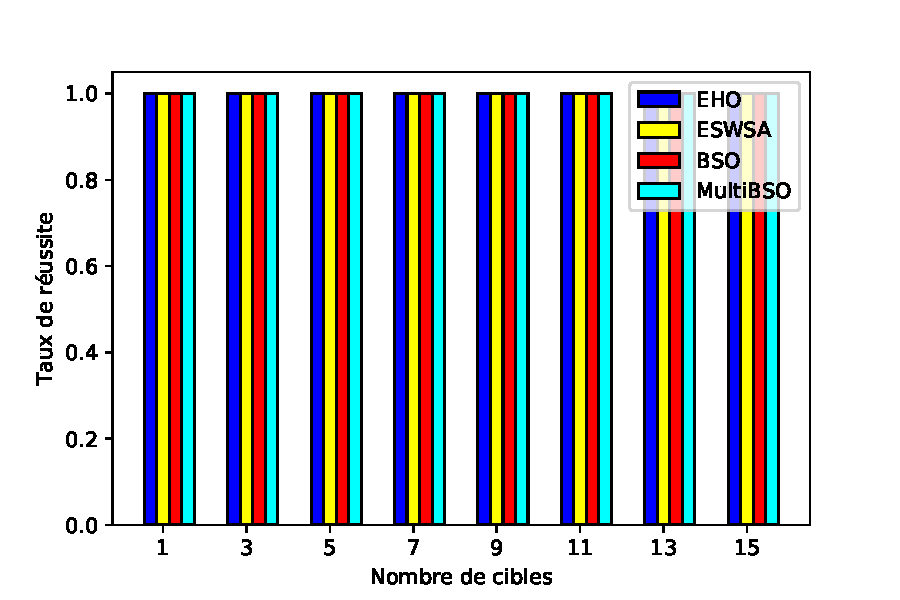
\includegraphics[width=\textwidth]{SansObs/BarChart/TauxNbTarget.pdf}}
		\captionof{figure}{Comparaison de la variation du taux de réussite des algorithmes selon le nombre de cibles.}
		\label{TN}
	\end{minipage}\hfill
	
	\subsubsection{Variation du nombre d'itérations et temps d'exécution}
	\paragraph{a- Environnements simples (sans obstacles)}
	\textbf{ }\\
	\noindent
	Les deux figures \ref{IN} et \ref{tN} ci-dessous retracent la variation du nombre moyen d'itérations et temps moyen d'exécution de nos algorithmes confrontés à un nombre croissant de cibles dans des environnements sans obstacles.\\
	\vspace{-0.2cm}
	
	Tous les algorithmes résolvent le problème de recherche de cibles en un nombre d'itérations variant entre 1 à 31 itérations, à l'exception de BSO, qui vient bien après ses concurrents, démarrant de 8 et arrivant jusqu'à 83 itérations. Notons que la meilleure performance est attribuée à ESWSA.\\
	\vspace{-0.2cm}
	
	Nous avons obtenu des temps d'exécution remarquablement réduits pour l'ensemble des méthodes, certes les temps ont accru avec l'augmentation du nombre de cibles, mais cela reste très raisonnable entre 0.02 et 0.05 secondes pour ESWSA, entre 0.001 et 0.06 secondes pour Multi-BSO, de 0.01 à 0.07 secondes pour BSO et enfin, de 0.01 à 0.12 secondes pour ce qui est d'EHO.
	
	
	
	
	\noindent
	\begin{minipage}[t]{0.55\textwidth}
		\captionsetup{width=0.8\linewidth}
		\centering\raisebox{\dimexpr \topskip-\height}{%
			\includegraphics[width=\textwidth]{SansObs/LineChart/IterNbTarget.pdf}}
		\captionof{figure}{Comparaison de la variation du nombre d'itérations des algorithmes selon le nombre de cibles (sans obstacles).}
		\label{IN}
	\end{minipage}\hfill
	\hspace{-0.5cm}
	\begin{minipage}[t]{0.55\textwidth}
		\captionsetup{width=0.8\linewidth}
		\centering\raisebox{\dimexpr \topskip-\height}{%
			\includegraphics[width=\textwidth]{SansObs/LineChart/TimeNbTarget.pdf}}
		\captionof{figure}{Comparaison de la variation du temps d'exécution des algorithmes selon le nombre de cibles (sans obstacles).}
		\label{tN}
	\end{minipage}\hfill
	
	
	
	\paragraph{b- Environnements avec obstacles}
	\textbf{ }\\
	\noindent
	
	Les deux figures \ref{INo} et \ref{tNo}, décrivent la variation du nombre d'itérations et temps d'exécution de nos quatre approches à la recherche d'un nombre variable de cibles dans des environnements avec obstacles.\\
	\vspace{-0.2cm}
	
	Le nombre d'itérations croît avec l'augmentation du nombre de cibles dans l'environnement, BSO connaît la plus grande croissance en passant de 23.53 à 104.43 itérations. Multi-BSO fait moins d'itérations avec entre 6.10 et 26.08. EHO et ESWSA effectuent de 1.55 à 17.98 et de 2.58 à 7.58 itérations respectivement.\\
	\vspace{-0.2cm}
	
	Les temps d'exécution sont très courts pour l'ensemble des méthodes, notons l'augmentation des temps de 0.02 jusqu'à 0.48 secondes pour ESWSA. Ce dernier étant considéré comme le plus long, puis de 0.01 à 0.07 secondes pour EHO et de 0.01 à 0.05 pour les algorithmes inspirés des abeilles (BSO et Multi-BSO). 
	
	
	\noindent
	\hspace{-0.5cm}
	\begin{minipage}[t]{0.55\textwidth}
		\captionsetup{width=0.8\linewidth}
		\centering\raisebox{\dimexpr \topskip-\height}{%
			\includegraphics[width=\textwidth]{AvecObs/LineChart/IterNbTarget.pdf}}
		\captionof{figure}{Comparaison de la variation du nombre d'itérations des algorithmes selon le nombre de cibles (avec obstacles).}
		\label{INo}
	\end{minipage}\hfill
	\begin{minipage}[t]{0.55\textwidth}
		\captionsetup{width=0.8\linewidth}
		\centering\raisebox{\dimexpr \topskip-\height}{%
			\includegraphics[width=\textwidth]{AvecObs/LineChart/TimeNbTarget.pdf}}
		\captionof{figure}{Comparaison de la variation du temps d'exécution des algorithmes selon le nombre de cibles (avec obstacles).}
		\label{tNo}
	\end{minipage}\hfill
	
	
	
	
	
	\paragraph{c- Environnements complexes}
	\textbf{ }\\
	\noindent
	
	Les \textit{diagrammes à lignes brisées} des figures \ref{INc} et \ref{tNc} mettent en relief l'influence du nombre de cibles recherchées sur le nombre d'itérations et temps d'exécution de nos algorithmes, dans des environnements complexes.\\
	\vspace{-0.2cm}
	
	En observant le nombre d’itérations, nous constatons que nos approches peuvent être classées en fonction de leur rythme de croissance face au nombre de cibles recherchées. Telles que, BSO possède les plus grands nombres avec de 25.53 à 125.83 itérations, puis vient Multi-BSO qui passe de 8.73 à 35.28 itérations, suivies d'EHO dont les nombres sont entre 1.8 et 21.3 itérations, non loin ESWSA avec entre 2.45 et 20.78 itérations.\\
	\vspace{-0.2cm}
	
	Les algorithmes inspirés des abeilles possèdent des temps d'exécution bas, légèrement croissant avec l'augmentation du nombre de cibles passant de 0.01 à 0.05 secondes. EHO s'en rapproche avec une croissance de ses temps allant de 0.001 à 0.08 secondes. ESWSA quant à lui sort du lot avec une augmentation de 0.02 à 0.48 secondes.
	
	\noindent
	\begin{minipage}[t]{0.54\textwidth}
		\captionsetup{width=0.8\linewidth}
		\centering\raisebox{\dimexpr \topskip-\height}{%
			\includegraphics[width=\textwidth]{Complex/LineChart/IterNbTarget.pdf}}
		\captionof{figure}{Comparaison de la variation du nombre d'itérations des algorithmes selon le nombre de cibles (complexe).}
		\label{INc}
	\end{minipage}\hfill
	\hspace{-0.5cm}
	\begin{minipage}[t]{0.54\textwidth}
		\captionsetup{width=0.8\linewidth}
		\centering\raisebox{\dimexpr \topskip-\height}{%
			\includegraphics[width=\textwidth]{Complex/LineChart/TimeNbTarget.pdf}}
		\captionof{figure}{Comparaison de la variation du temps d'exécution des algorithmes selon le nombre de cibles (complexe).}
		\label{tNc}
	\end{minipage}\hfill
	
	
	
	\subsubsection{Analyse relative au nombre de cibles}
	D'après les résultats présentés ci-dessus par rapport au nombre de cibles recherchées dans les différents types d'environnements expérimentés, nous sommes en mesure de tirer les quelques conclusions qui suivent :
	
	\begin{itemize}
	\item[$\bullet$] Nos quatre méta-heuristiques ont fait leurs preuves de par leur capacité à trouver toutes les cibles qu'importe leur nombre (selon les conditions citées).
		
	\item[$\bullet$] Plus il y a de cible à chercher, plus les algorithmes font d'itérations et plus le temps d'exécution croît.
		
     \item[$\bullet$] BSO détient le plus grand nombre d'itérations quel que soit l'environnement, mais en contrepartie il possède les meilleurs temps d'exécution.
    
     \item[$\bullet$] La méta-heuristique ESWSA effectue des temps acceptables dans des environnements simples à grand nombre de cibles avec un nombre d'itérations record. En revanche, lors de la présence d'obstacles les temps d'exécution deviennent beaucoup trop importants comparés aux autres approches (BSO, EHO, Multi-BSO) détenant ainsi les pires temps.
     
     \item[$\bullet$] Quant aux deux autres algorithmes leur évolution en termes de temps et nombre d’itérations est bornée par celles de BSO et ESWSA.

		
	\item[$\bullet$] Le nombre d'itérations reste relativement acceptable pour 15 cibles, à noter qu'ESWSA, EHO et Multi-BSO étaient plus performants sur ce plan.
		
	\item[$\bullet$] Les temps d'exécution étaient globalement satisfaisants pour tous les algorithmes, car n'excédant pas les 0.5 secondes. 
		
	\item[$\bullet$] La densité des environnements en obstacles, joue un rôle important dans le comportement de nos approches, telle que, plus nos environnements sont complexes plus nos approches produisent d'efforts et prennent de temps à atteindre les cibles.
	\end{itemize}
	
	
	%%%%%%%%%%%%%%%%%%%%%%%%%%%%%%%%%%%%%%%%%%%%%%%%%%%%%%%%%%%%%%%%%%%%%%%%%%%%%%%%%%%%%%%%%%%%%%%%%%%%%%%%%%%%%%%%%%%%%%%%%%%%%%%%%%%%%%%%%%%%%%%%%%%%%%%%%%%%%%%%%%%%%
	
	
%	\newpage
	
	
	
	
	\subsection{Comparaison des types d'environnement}
	La moyenne des temps d'exécution et nombre d'itérations croît lors du passage d'environnements simples (sans obstacles) aux environnements avec obstacles, mais elles connaissent une considérable augmentation lorsqu'on a affaire à des environnements complexes.
	
	Cela est dû à la complexité des environnements entravant et rendant plus difficile le mouvement des robots, ainsi le choix de la bonne trajectoire devient de plus en plus complexe ce qui impacte le temps d'exécution.\\
	Pour ce qui est des taux de réussite, ils dépendent beaucoup plus des méthodes de recherche.
	
	\subsection{Comparaison de nos quatre approches}
	Nos quatre approches développées et testées ne possèdent pas les mêmes comportements faces aux différentes variantes liées à l'environnement de recherche. Nous pouvons conclure que :
	\begin{itemize}
		\item[$\bullet$] L'approche Multi-BSO est la plus stable, les variations du nombre d'itérations et de temps d'exécution sont harmonieux.
		
		
		\item[$\bullet$] L'algorithme ESWSA est le meilleur en termes de nombre d'itérations suivi de près par EHO. 
		
		\item[$\bullet$] Les méta-heuristiques inspirées des abeilles sont les meilleurs en termes de temps d'exécution.
		
		\item[$\bullet$] L'algorithme ESWSA atteint parfois des temps d'exécution peu raisonnables.
		
		\item[$\bullet$] Globalement le multi-swarming (Multi-BSO) a grandement amélioré BSO que ce soit dans les taux de réussite, le nombre d'itérations ou temps d'exécution. 
		
		\item[$\bullet$] BSO et Multi-BSO ont quelques lacunes par rapport aux très grands environnements.
		
		\item[$\bullet$] EHO possède le meilleur compromis entre taux de réussite (toujours à 100\%), nombre d'itérations assez bas et temps d'exécution très raisonnables.
		
	\end{itemize}
	
	
	
	%%%%%%%%%%%%%%%%%%%%%%%%%%%%%%%%%%%%%%%%%%%%%%%%%%%%%%
	%%%%%%%%%%%%%%%%%%%%%%%%%%%%%%%%%%%%%%%%%%%%%%%%%%%%%%
	%%%%%%%%%%%%%%%%%%%%%%%%%%%%%%%%%%%%%%%%%%%%%%%%%%%%%%
	
	
	\section{Simulateur}
	La réalisation de notre simulateur temps réel et interactif pour la visualisation de l'évolution des approches implémentées que ça soit BSO, Multi-BSO, EHO ou encore ESWSA, a été mise en œuvre afin de faciliter la compréhension de notre travail.
	
	\subsection{Fonctionnement}
	\noindent
	L'affichage de l'environnement de recherche de notre simulateur passe par les étapes suivantes :
	\begin{itemize}
		\item[$\bullet$] Sélection de l'environnement à explorer sous sa forme matricielle comme décrite dans la modélisation de la section \ref{vuEnv}.
		
		\item[$\bullet$] Translation de l'espace de recherche sélectionné en une image PNG, en assignant aux obstacles et à la portée deux couleurs distinctes.
		
		\item[$\bullet$] Représentation de chaque position de l'environnement de recherche par un unique pixel dans l'image PNG.\\
	\end{itemize}
	
	Quant à l'étape de recherche des cibles, elle nécessite de retracer la trajectoire de chaque robot, en dessinant leurs chemins entre la position actuelle et la nouvelle position calculée par la méta-heuristique de recherche, le dessin suit l'algorithme de BRESENHAM \cite{line}. \\
	
	Dans notre simulateur temps réel, pour une question de fluidité et de parallélisme, il est nécessaire de faire appel au \textit{multi-threading}, un \textit{thread} pour l'exécution de la méta-heuristique et un autre pour l'interface de simulation, la coordination entre ces deux \textit{threads} est illustrée par le schéma de la figure \ref{sim} qui suit.

	\noindent
	\begin{center}	  
		\captionsetup{width=0.8\linewidth}
		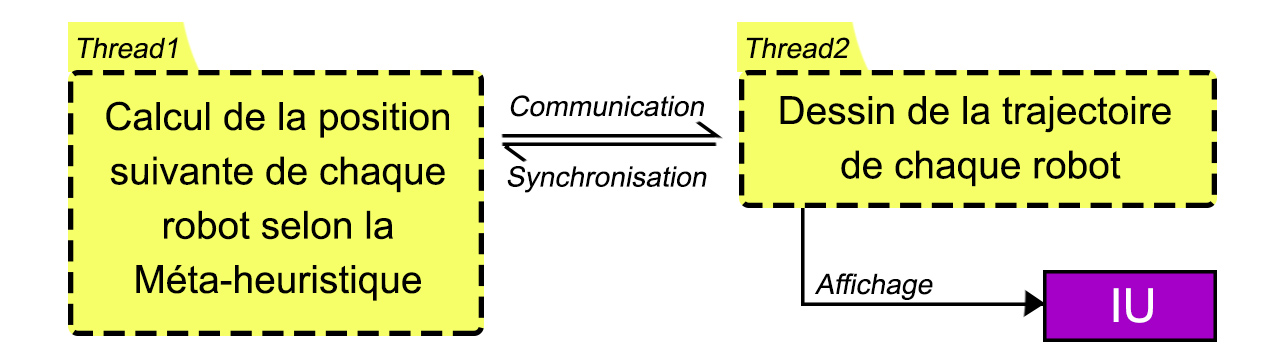
\includegraphics[width=0.8\textwidth]{threads.jpg}%
		\captionof{figure}{Schéma de communication du système multi-threads.}\label{sim}%
	\end{center}
	

	\subsection{Interface}
	L'interface offre deux sections possibles, une dédiée au choix de l'environnement nous permettant de choisir un environnement selon nos préférences et paramètres, celle-ci est représentée dans la figure \ref{uienv} ci-dessous :
	
	\begin{center}	  
		\captionsetup{width=1\linewidth}
		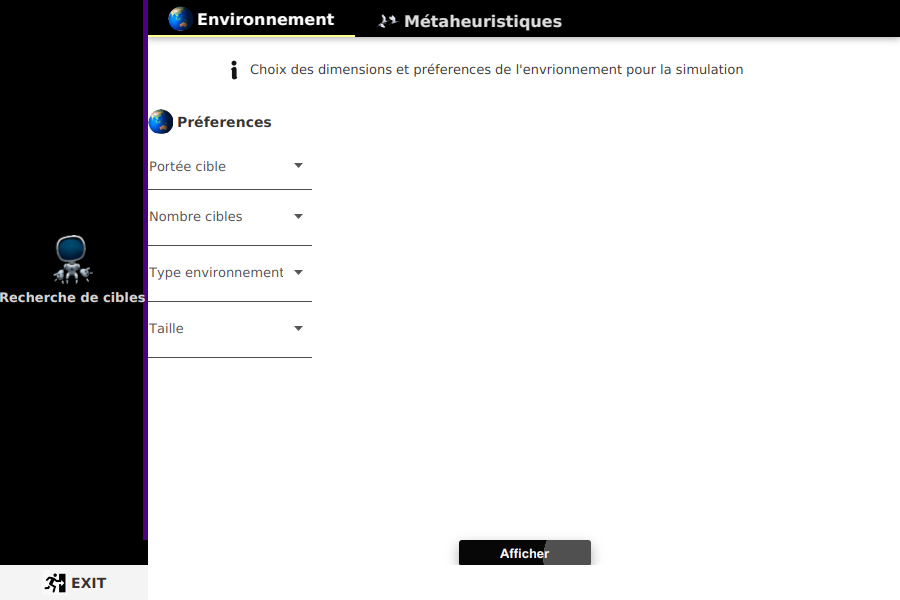
\includegraphics[scale=0.45]{screens/env.png}%
		\vspace{-0.1 cm}
		\captionof{figure}{Présentation de l'interface}\label{uienv}%
	\end{center}
	
	Et une autre section dédiée aux méta-heuristiques, qui englobe toutes les approches basées essaims traitées dans ce projet, afin d'être appliquées à l'environnement choisi dans la section Environnement. 
	Cette section est visible dans la figure \ref{uimeta} qui suit :
	
	\begin{center}	  
		\captionsetup{width=1\linewidth}
		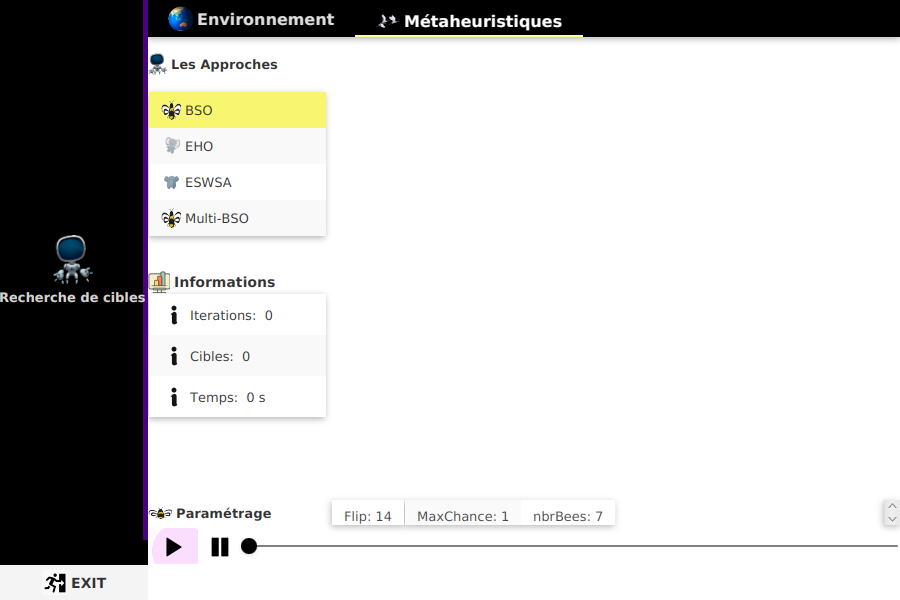
\includegraphics[scale=0.45]{screens/metaheuristiques.png}%
		\vspace{-0.1 cm}
		\captionof{figure}{Présentation de la section Métaheuristiques}\label{uimeta}%
	\end{center}
	
	\subsubsection{Environnement}
	La section Environnement permet à l'utilisateur de choisir un environnement selon les paramètres et préférences suivantes :
	
	
	
	\paragraph{Nombre de cibles}
	Nos environnements peuvent comporter une ou plusieurs cibles dont les positions sont générées de manière aléatoire.
	
	Dans le cadre de notre simulation, nous nous sommes contentés de permettre deux choix pour le nombre de cibles qui sont:
	\begin{itemize}
		\item [$\bullet$] Mono-cible : une seule cible.
		\item [$\bullet$] Multi-cibles : avec 5 cibles.
	\end{itemize}
	Ce choix peut être augmenté selon le nombre de cibles souhaité.
	

	
	\paragraph{Portée des cibles}
	Les portées de cibles disponibles dans l'application sont donc catégorisées comme suit :
	\vspace{0.3cm}
	\begin{itemize}
		\item [$\bullet$] \textbf{Portée petite}, d'un rayon d'environ 5\% de la taille de l'environnement.
		\item [$\bullet$] \textbf{Portée moyenne}, d'un rayon d'environ 15\% de la taille de l'environnement.
		\item [$\bullet$] \textbf{Portée large}, d'un rayon d'environ 25\% de la taille de l'environnement.
	\end{itemize}
	
	\paragraph{Types d'environnements}
	Les types d'environnements simples, avec obstacles et complexes sont représentés dans la figure \ref{typss}, sont mis à disposition. Dans le cas des deux derniers types d'environnements, il est à noter que les positions et distributions des obstacles sont générées aléatoirement.
		
		\newpage
	\noindent
	%\hspace{-0.5cm}
	\begin{center}
	
%	\begin{figure}[h]
	\begin{multicols}{3}
		\begin{minipage}[t]{0.3\textwidth}
			\centering\raisebox{\dimexpr \topskip-\height}{%
				
\includegraphics[width=\textwidth]{envSpml.png}}
			\xdash[3.5cm]
			Environnement simple
		\end{minipage}\hfill
		\columnbreak
		\begin{minipage}[t]{0.3\textwidth}
			\centering\raisebox{\dimexpr \topskip-\height}{%
				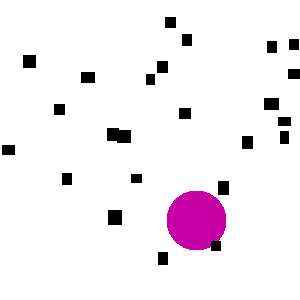
\includegraphics[width=\textwidth]{envObs.png}}
			
			\xdash[3.5cm]
			Environnement à obstacles\\
		\end{minipage}\hfill
		\columnbreak
		\begin{minipage}[t]{0.3\textwidth}			
			\centering\raisebox{\dimexpr \topskip-\height}{%
				\includegraphics[width=\textwidth]{envCmpl.png}}
			
			\xdash[3.5cm]
			Environnement complexe
		\end{minipage}\hfill
	\end{multicols}
%	\end{figure}
	\captionof{figure}{Les types d'environnements possibles.}\label{typss}
\end{center}
	
	
	
	
	\paragraph{Taille d'environnement}
	Les environnements varient selon leur taille, on a alors choisi à titre représentatif quelques tailles par classe, telles que :
	\begin{itemize}
		\item  [$\bullet$]100 et 400 qui sont assez petits.
		\item  [$\bullet$]600 et 1000 dits de taille moyenne.
		\item  [$\bullet$]1500 qui est assez grand.
	\end{itemize}
	
	\paragraph{Afficher}
	La section environnement présentée dans la figure \ref{uienvsetting} comporte le bouton \textit{afficher} qui sert à visualiser l'environnement choisi en fonction des préférences insérées dans les listes de choix multiples de chaque influent (portée, nombre cibles, ...). 
	
	Ci-dessous un exemple d'environnement sélectionné :
	\begin{center}	  
		\captionsetup{width=1\linewidth}
		\includegraphics[scale=0.48]{screens/envsetting.png}%
		\vspace{-0.1 cm}
		\captionof{figure}{Affichage de l'environnement selon les préférences insérées}\label{uienvsetting}%
	\end{center}
	
	\subsubsection{Métaheuristiques}
	
	\paragraph{Les approches}
	Les approches basées essaims auxquels nous avons eu affaire tout au long de ce mémoire \textit{BSO, EHO, ESWSA} et \textit{Multi-BSO} y sont proposées sous forme d'une liste permettant de choisir celle à exécuter.
	Une fois qu'on clique sur une approche deux possibilités pour le choix du paramétrage s'offrent à nous:
	
	
	\paragraph{- Paramétrage avec algorithme génétique}
	L'option de paramétrage avec l'algorithme génétique (Mini-GA incrémental) est accessible pour chaque approche, comme le montre la figure \ref{uiga} ci-dessous.
	
	\begin{center}	  
		\captionsetup{width=1\linewidth}
		\includegraphics[scale=0.5]{screens/bsoautoparam.png}%
		\vspace{-0.1 cm}
		\captionof{figure}{Auto-paramétrage avec l'algorithme génétique}\label{uiga}%
	\end{center}
	
	\paragraph{- Paramétrage manuel}
	Le paramétrage manuel se fait en choisissant pour chaque paramètre de l'approche basée essaim une valeur.
	Les figures \ref{uibso} et \ref{uibsoga} ci-dessous illustrent ces paramètres pour BSO.
	
	\begin{minipage}{0.5\textwidth}
		\centering
		\includegraphics[scale=0.50]{screens/bsopopmenu.png}%
		\vspace{-0.1 cm}
		\captionof{figure}{Menu de paramétrage}\label{uibso}%
	\end{minipage}%
	\begin{minipage}{0.5\textwidth}
		\centering	  
		\captionsetup{width=0.6\linewidth}
		\includegraphics[scale=0.40]{screens/bsoparam20-2-3.png}%
		\vspace{-0.1 cm}
		\captionof{figure}{Menu de paramétrage manuel pour BSO}\label{uibsoga}%
	\end{minipage}
	
	\textbf{ }\\
	
	\noindent
	\begin{minipage}{0.6\textwidth}
		\paragraph{Les informations}
		Ce sont les détails identiques pour chaque approche et qui sont :
		\textit{Nombre d'itérations, Nombre de cibles trouvées, Temps d'exécution (sec)} comme présentés dans la figure \ref{bsoinfo}.
		
		Ces informations sont mises à jour en temps réel,  c'est-à-dire qu'elles sont modifiées à chaque itération (le nombre d'itérations inclus).
	\end{minipage}
	\begin{minipage}{0.4\textwidth}
		\captionsetup{width=0.7\linewidth}
		\centering
		\includegraphics[scale=0.55]{screens/bsoinfo.png}%
		\vspace{-0.1 cm}
		\captionof{figure}{Informations durant l'exécution de BSO}\label{bsoinfo}%
	\end{minipage}
	
	
	
	
	
	\paragraph{Paramétrage} est une liste horizontale comme illustrée dans la figure \ref{listparam}, elle contient les paramètres de l'exécution de l'approche choisie, qu'elle soit générée par algorithme génétique ou bien manuellement.
	
	
	\begin{center}	  
		\captionsetup{width=1\linewidth}
		\includegraphics[scale=0.65]{screens/bsoparamlist.png}%
		\vspace{-0.1 cm}
		\captionof{figure}{Liste des paramètres pour BSO}\label{listparam}%
	\end{center}
	
	
	%\paragraph{Les boutons}
	%\textbf{ }\\
	%Notre interface comporte deux boutons qui se trouvent à côté du "slider".
	\paragraph{Start}
	Le bouton \textit{"Start"} \includegraphics[scale=0.55]{screens/start.png} , permet de débuter l'exécution après avoir choisi l'approche.
	Ainsi, l'image de l'environnement et des robots (abeilles ou éléphants) sur l'environnement s'affichent.
	
	
	\paragraph{Stop}
	Le bouton \textit{"Stop"}	\includegraphics[scale=0.55]{screens/stop.png}, permet d'arrêter et mettre fin à l'exécution de l'approche, afin de choisir une autre méta-heuristique à exécuter ou bien relancer la même avec d'autres paramètres.
	
	
	\paragraph{Le slider} de la figure \ref{slider} joue le rôle d'une barre de progression, tel qu'il s'incrémente après chaque itération de l'approche en cours d'exécution. Une fois l'exécution terminée, il permet de revenir en arrière retraçant ainsi la trajectoire des robots dans l'environnement. Comme pour un film ou une vidéo, nous avons la possibilité d'avancer du début jusqu'à la fin, pour revoir l'exécution.
	\begin{center}	  
		\captionsetup{width=1\linewidth}
		\includegraphics[scale=0.5]{screens/slider.png}%
		\vspace{-0.3 cm}
		\captionof{figure}{Le slider}\label{slider}%
	\end{center}
	
	L'illustration \ref{bsorun} suivante est un exemple d'une exécution de BSO dans un environnement multi-cibles de petites portées et avec obstacles.
	\begin{center}	  
		\captionsetup{width=1\linewidth}
		\includegraphics[scale=0.48]{screens/bsorun20-2-3.png}%
		\vspace{-0.3 cm}
		\captionof{figure}{Exemple d'exécution de BSO.}\label{bsorun}%
	\end{center}
	
	
	\paragraph{Quitter}
	Un bouton \textit{"Quitter"} \includegraphics[scale=0.6]{screens/exit.png} se trouve en bas à gauche de l'interface, il permet de sortir de l'application dès que nous le souhaitons.
	
	
	%	\begin{center}	  
	%		\captionsetup{width=1\linewidth}
	%		\includegraphics[scale=0.8]{screens/exit.png}%
	%		\vspace{-0.1 cm}
	%		\captionof{figure}{Bouton pour quitter l'application}\label{exit}%
	%	\end{center}
	
	
	
	
	
	
	\section{Conclusion}
	
 À travers ce chapitre, on a pu discuter et effectuer une multitude de tests expérimentaux qui concernent toutes les approches de résolution d'intelligence en essaim implémentées qu'on cite 
 BSO, Multi-BSO, EHO et ESWSA.
 D'autres tests ont été présentés portant sur l'algorithme génétique qui ont comme objectif d'effectuer un réglage de paramètres des algorithmes implémentés.
 
 La série de tests relative à l'environnement (23 040 exécutions) a touché à plusieurs caractéristiques comme \textit{La portée de la cible, la taille de l'environnement, nombre de cibles ainsi que la densité des obstacles.} 
 L'analyse de l'ensemble des résultats nous a permis d'observer les changements de comportement des algorithmes, ce qui nous a aidées à extraire les avantages de chaque approche, ainsi que leurs inconvénients tout en justifiant les causes.
 
 Ainsi, nous envisageons une hybride qui peut éventuellement surpasser les algorithmes vus dans ce mémoire, cela en combinant leurs points forts et remédiant à leurs points faibles.
 

